\documentclass[10pt, openany]{book}

\usepackage[T1]{fontenc}
\usepackage[utf8]{inputenc}
\usepackage[english]{babel}
\usepackage{geometry}
\usepackage{graphicx}
\usepackage[pdfa=true]{hyperref}
\usepackage{cite}
\usepackage{listings}
\usepackage[printonlyused,withpage]{acronym}
\usepackage{siunitx}
\usepackage{multirow}
\usepackage{setspace}
\usepackage{xcolor}
\usepackage{listings}
\usepackage{minted}
\usepackage{tabularx}
\usepackage{marvosym}
\usepackage{svg}
\usepackage{amsmath}
\usepackage{amsthm}
\usepackage{pseudo}
\usepackage{pifont}
\newcommand{\cmark}{\ding{51}}
\newcommand{\xmark}{\ding{55}}
\usepackage{stmaryrd}
\newcommand{\assignment}[1]{\llbracket #1 \rrbracket}
\usepackage{wrapfig}
\usepackage{amsfonts}


\newtheorem{theorem}{Theorem}
\newtheorem{definition}{Definition}

%--- pdf/a format ----
% insert metadata about the document here
% \RequirePackage{filecontents}
% \begin{filecontents*}{\jobname.xmpdata}
% \Title{Document’s title}
% \Author{Author’s name}
% \Language{en-US}
% \Subject{The abstract, or short description.}
% \Keywords{keyword1\sep keyword2\sep keyword3}
% \end{filecontents*}
\usepackage{colorprofiles}
\usepackage[a-1b,mathxmp]{pdfx}[2018/12/22]
\usepackage[T1]{fontenc}
\hypersetup{pdfstartview=}


%
% This is the official thesis template of
% the Institute of Computer Science at the
% Georg-August-University of Göttingen
%
%      author: kellner@cs.uni-goettingen.de
% last update: 17/02/2015
%
% If you find any sort of mistake please let me know
% so that it can be fixed in future releases.
%


%--- include custom commands ---
%
% own commands
%

%double empty page
\newcommand \myemptypage {
    \clearpage
    \thispagestyle{empty}
    \null
    \cleardoublepage
}

%create abstract environment that is not available in latex book style
\newcommand\abstractname{Abstract}
\newenvironment{abstract}{%
    \begin{center}%
        \normalfont\Large\bfseries \abstractname
    \end{center}%
    \it%
    }
    {}


%--- include general configuration ---
%
% general configuration
%

% Palatino font as serif font
\usepackage{palatino}
\linespread{1.05}
% Helvatica font as sans-serif
\usepackage{helvet}
% Use microtype to improve typesetting
\usepackage{microtype}

%set page margin for DIN A4
\geometry{a4paper, left=2.5cm, right=2.5cm, top=4cm, 
          bottom=5cm, bindingoffset=1cm}

%makes TeX less fussy about line breaking
\sloppy

% Replacement for changing parskip and parindent directly
\usepackage{parskip}

%1.5 spacing
\onehalfspacing
{}

% Make chapter heading smaller
\usepackage{titlesec}
\titleformat{\chapter}[display]
  {\LARGE\bf}{\chaptertitlename\ \thechapter}{10pt}{\huge\bf}

%define some colors
\definecolor{darkblue}{rgb}{0.0,0.0,0.5}
\definecolor{grey}{rgb}{0.8,0.8,0.8}
\definecolor{lightgrey}{rgb}{0.95,0.95,0.95}

%set listing style properties for python
\lstset{language=Python,
    basicstyle=\footnotesize\ttfamily,
    captionpos=b,
    frame=tb,
    commentstyle=\color{gray} \bfseries,
    stringstyle=\color{green}\ttfamily,
    keywordstyle=\color{darkblue}\bfseries,
    breaklines=true,
    aboveskip=10mm,
    belowskip=10mm,
    showstringspaces=false
    numbers=left,
    %stepnumber=5,
    numberstyle=\tiny,
    numbersep=5pt
}


%override reference title and listings title
\renewcommand \bibname{References}
\renewcommand{\lstlistlistingname}{List of Listings}




%--- basic document configuration ---
\newcommand{\mytype}{Master's Thesis}
%\newcommand{\mytype}{Master's Thesis}

\newcommand{\mycourse}{Applied Computer Science}
%\newcommand{\mycourse}{Internet Technologies and Information Systems}

\newcommand{\mytitle}{A functional solver for word equations with regular constraints}
\newcommand{\myauthor}{Maximilian David Eipper}
\newcommand{\mydepartment}{Institute of Computer Science}
\newcommand{\mysubmissiondate}{31st of March 2023}
%\newcommand{\mythesisid}{201x-xx} %assigned by examination office
\newcommand{\myfirstsupervisor}{Prof. Dr. Florin Manea}
\newcommand{\mysecondsupervisor}{Dr. Henrik Brosenne}

\newenvironment{allintypewriter}{\ttfamily}{\par}

\begin{document}

 \pagenumbering{roman}
    \setcounter{page}{1}

    %--- cover page ---
    %
% title page
%

\begin{titlepage}
    %--- logo ---
    \normalsize
    \begin{tabularx}{\textwidth}{lXr}
        \multirow{2}{*}{
\includegraphics[width=6.5cm]{images/goe-logo.jpg}} 
        & & \\
    \end{tabularx}

    %default settings for the rest
    \large
    \centering

    \vspace{3cm}

    \textbf{\LARGE \mytype}\\

    submitted in partial fulfillment of the\\
    requirements for the course ``\mycourse''

    \vspace{2cm}

    \textbf{\LARGE \mytitle}

    \vspace{2cm}

    \myauthor

    \vspace{2cm}

    \mydepartment

    \vspace{2cm}

    Bachelor's and Master's Theses\\
    of the Center for Computational Sciences\\
    at the Georg-August-Universität Göttingen

    \vspace{0.2cm}

    \mysubmissiondate


    %--- new page ---
    \myemptypage
    \clearpage
    \thispagestyle{empty}
    \null
    \flushleft
    \onehalfspacing
    \normalsize

    \vspace{12cm}

    Georg-August-Universität Göttingen\\
    Institute of Computer Science\\[3ex]
    Goldschmidtstraße 7\\
    37077 Göttingen\\
    Germany\\[3ex]

    \begin{tabular}{@{}ll}
        \Telefon & +49 (551) 39-172000\\
        \fax & +49 (551) 39-14403\\
        \Letter & \href{mailto:office@informatik.uni-goettingen.de}{office@informatik.uni-goettingen.de}\\
        \Mundus & \url{www.informatik.uni-goettingen.de}\\
    \end{tabular}

    \vspace{1.0cm}

    \begin{tabular}{@{}ll}
        First Supervisor: & \myfirstsupervisor\\
        Second Supervisor:& \mysecondsupervisor\\
    \end{tabular}

    \clearpage
\end{titlepage}


    % \myemptypage

    %--- statement page ---
    \thispagestyle{empty}

\null
\vspace{16.5cm}

\rule{\textwidth}{0.4pt}

I hereby declare that I have written this thesis independently without any help from others and without the use of documents or aids other than those stated. I have mentioned all used sources and cited them correctly according to established academic citation rules.

\vspace{0.2cm}

Göttingen, \mysubmissiondate

    % \myemptypage

    %--- abstract ---
    \clearpage\phantomsection\pdfbookmark{\abstractname}{abstract}
    \thispagestyle{empty}
    \begin{abstract}
    We present a prefix-based approach for solving regex-constrained word equations combining the Nielsen transformation and Brzozowski derivatives. Differently from most approaches, we solve the word equation and the regex constraints in a combined manner. We provide a Haskell implementation of a solver using our approach. Our implementation outperforms state-of-the-art solvers on regex-constrained, quadratic equations.
    Since our approach is only viable within this particular niche, we conclude it is best suited as a solver tactic, as opposed to a standalone solver.
\end{abstract}

    % \myemptypage

    %reset acronyms after abstract
    \acresetall

    %--- table of contents ---
    \clearpage\phantomsection\pdfbookmark{\contentsname}{toc}
    \tableofcontents
    % \myemptypage

    %--- list of figures ---
    %\listoffigures
    %\myemptypage

    %--- list of tables ---
    %\listoftables
    %\myemptypage

    %--- list of listings ---
    %\lstlistoflistings
    %\myemptypage

    %--- list of acronyms ---
    %\chapter*{List of Abbreviations}

\begin{acronym}[myacronyms]
    \acro{FYI}{For Your Information}    
\end{acronym}

    %\myemptypage


    %arabic page numbers
    \pagenumbering{arabic}
    \setcounter{page}{1}
    
    \chapter{Introduction}

The field of string solving deals with finding solutions for string-related problems, where \textit{strings} are sequences of symbols.
These problems can take many forms, but they often involve finding patterns, checking some properties of the strings or transforming the strings in some way.

This includes but is not restricted to:
\begin{itemize}
    \item sorting strings by an ordering relation, such as lexicographic order
    \item finding out if a string contains a specific word
    \item finding out if a string follows a specific pattern
    \item compressing/decompressing a string to store it efficiently
    \item checking the syntax of a string to ensure that it follows certain rules, such as those of a programming language or a formal language
    \item solving equations where the variables take string values
\end{itemize}

String solving is an active area of research with many open problems still to be explored. It has a wide range of applications in computer science as well as in related fields.

In this work, we will focus on the last problem: Solving equations of strings. This problem does not deal with numeric equations but instead with so-called \textit{word equations} in which the variables take symbolic values from the monoid $\Sigma^*$. Consider the equation $abxb = ybx$ where $a$ and $b$ are terminal symbols from $\Sigma$ and $x$ and $y$ are variables that can take any string value. This equation is satisfied for $x = b, y = ab$. Let us consider another equation: $xa = byx$. It does not have a solution because no matter which values we choose for $x$ and $y$ the two sides are never equal.

Usually, we add additional rules -- so-called \textit{constraints} -- to the variables. One such constraint could be that $x$ must be at most 10 characters long or $y$ must satisfy the regular expression $ab*$.

Word equations are used to model problems in cyber security and formal verification. In the former, problems can be modeled in a way so that the solutions to the equations correspond with attack vectors that can be used to breach security.

This work will deal with one specific subproblem of solving word equations. We will solve word equations where the variables have regular expression constraints. For this, we take Nielsen's algorithm \cite{nielsen1917} for solving word equations without constraints and extend it with Brzozowski's notion of regex derivatives \cite{brzozowski} to solve equations with regex constraints.
To test the viability of our approach, we provide a Haskell implementation of a string solver that follows this method. We benchmark against the state-of-the-art solvers CVC \cite{cvc4,cvc5} and Z3 \cite{z3} to find out under which circumstances our approach can compete with them.

Usually, string solvers solve word equations and regex constraints separately. We are aware of only one approach -- Noodler \cite{noodler} -- that solves equations and constraints in a joined manner by using an automata structure. Our contribution is to provide a second approach that solves equations and constraints together by using the Nielsen transformation and Brzozowski derivatives. The goal of this work is to present an algorithm, provide an implementation and evaluate its performance.

This thesis is structured as follows. In chapter \ref{ch_foundations}, we introduce some basic notation and give a rough overview of string solving and related strategies. Subsequently, we have a detailed look at the Nielsen transformation and Brzozowski's algorithm for regex matching.
In chapter \ref{ch_approach}, we present our modification to the Nielsen transformation to extend it to regex-constrained variables and prove its correctness.
In chapter \ref{ch_implementation}, we give a technical report on our Haskell implementation of the algorithm presented in chapter \ref{ch_approach}.
In chapter \ref{ch_benchmarks}, we explain the setup of our benchmarks. First, we present three benchmark sets. Then, we introduce the other string solvers we benchmark against. Finally, we explain how the experiment is going to be conducted.
In chapter \ref{ch_results}, we document and interpret the results of our benchmarks.
Finally, in chapter \ref{ch_conclusion}, we summarize our work, draw a conclusion from our findings in chapter \ref{ch_results} and give an outlook on future work.

    \chapter{Foundations} \label{ch_foundations}
\vspace{-0.45cm}
This chapter will introduce all theoretical foundations for our approach. We first introduce some notation. Then, we give an overview of the field of word equation solving, going into detail on the Nielsen transformation. Finally, we introduce some regex theories, focusing mainly on Brzozowski's work.

\section{Basics}
Words are sequences over a fixed length alphabet $\Sigma$. We write $w = w_1w_2...w_n, w_i \in \Sigma$. We denote the set of all words over $\Sigma$ as $\Sigma^*$, which forms a monoid under concatenation and the empty word $\varepsilon$. We define the length of a word $|w_1w_2...w_n| = n$.
While we use $\Sigma$ to denote the alphabet of terminal symbols, we use $X$ to denote the set of variables.
A word equation is an expression of the form $\alpha = \beta$ where $\alpha, \beta \in (\Sigma \cup X)^*$. If not specified differently, we use $a, b \in \Sigma, a \neq b$ and $x, y \in X, x \neq y$.

We define the replacement function $\varphi_{\cdot \rightarrow \cdot}(\cdot)$ so that $\varphi_{x \rightarrow \alpha}(\beta)$ denotes the result of replacing every occurrence of $x$ with $\alpha$ in $\beta$. E.g. $\varphi_{x \rightarrow ay}(xbbxy) = aybbayy$.
\[
\begin{tabular}{c c c}
    $\varphi_{x \rightarrow \alpha}(x)$ & $=$ & $\alpha$ \\
    $\varphi_{x \rightarrow \alpha}(y)$ & $=$ & $y$ \\
    $\varphi_{x \rightarrow \alpha}(a)$ & $=$ & $a$ \\
    $\varphi_{x \rightarrow \alpha}(\beta_1\beta_2...\beta_n)$ & $=$ & $\varphi_{x \rightarrow \alpha}(\beta_1)\varphi_{x \rightarrow \alpha}(\beta_2)...\varphi_{x \rightarrow \alpha}(\beta_n)$ \\
\end{tabular}
\]
Additionally, we introduce the prefix deletion function $\varphi_{DEL}$ with
\[
    \varphi_{DEL}(a\alpha) = \alpha
\]
Finally, for readability, we define the reverse order function composition $\circ'$ with
\[
    f \circ' g = g \circ f
\]

\section{Word Equations}

A word equation is an expression of the form $\alpha_1x_1\alpha_2x_2...x_{n-1}\alpha_n = \beta_1y_1\beta_2y_2...y_{m-1}\beta_m$ where $\alpha_i, \beta_i \in \Sigma^*, x_i, y_i \in X$. Now, the goal is to find out if there is an assignment function $\assignment{\cdot}: X \rightarrow \Sigma^*$ s.t. $\alpha_1\assignment{x_1}\alpha_2\assignment{x_2}...\assignment{x_{n-1}}\alpha_n = \beta_1\assignment{y_1}\beta_2\assignment{y_2}...\assignment{y_{m-1}}\beta_m \in \Sigma^*$. In other words, we are interested in finding a function that maps the variables to words in a way that makes both sides of the equation equal. Sometimes we might just be interested in finding out whether such a mapping exists without constructing it.

We consider two special cases of word equations: \textit{Quadratic} word equations and \textit{regular} word equations. Quadratic word equations are equations in which each variable occurs at most twice. For example, $xxy = ayz$ is quadratic, while $xxy = axz$ is not. Regular word equations are an even stricter subclass of quadratic word equations: Each variable may occur at most once on each side. $xy = ax$ is regular, while $xx = ay$ is not.

\section{Constrained Variables}
Until now, variables have always been \textit{unconstrained} in the way that they can take any values from $\Sigma^*$. This is not sufficient for many real-world applications. Modeling dates or passwords, for example, requires the variables to follow special formats, to have specific lengths or to be selected over only a subalphabet of $\Sigma$.

Instead of $x \in \Sigma^*$, we shall write $x \in \Sigma^k$ to denote variables whose values must be of length $k$. Similarly, we write $x \in \Sigma'^*$ for $\Sigma' \subset \Sigma$ to denote variables that only take symbols from a restricted subset of $\Sigma$.
For now, the only other kind of constraint we are interested in is regular expressions.

Let the notion $x \in ab*$ stand for the constraint that $x$ must match the regular expression $ab*$. This means $x$ can take the values $a, ab, abb, ...$ but not $b$ or $\varepsilon$. This work will focus on implementing regex constraints for variables in the Nielsen transformation. The reason for this is that regular expressions are generally expressive and that they prove powerful enough to cover most constraints presented in this chapter, albeit with drawbacks in usability or blowup in complexity. Subalphabets $\Sigma' = \{\sigma'_1, \sigma'_2, ... \sigma'_n\}$ can be modeled as one exhaustive disjunction over all terminal symbols of that subalphabet with $x \in \sigma'_1 | \sigma'_2 | ... | \sigma'_n$. This means that this simple constraint can only be modeled with linear complexity. Constant length constraints $x \in a^k$ can be modeled with $x \in \underbrace{aa...a}_{k}$. Again, we see linear blowup.
As regular languages are less powerful than context-free languages, complicated counting constraints where multiple variables depend on the same length constant $k$ cannot be modelled.

\section{Methods for Solving Word Equations} \label{methods}

To solve such equation problems, we can employ multiple different methods. This can involve manipulating the equation in various ways, such as substituting values for variables, rearranging terms, rewriting the equation in some way to simplify it or applying rules of algebra. Keep in mind that we are on a monoid, so basic tricks like adding an inverse do not work. Depending on the complexity of the equation and the methods used to solve it, solving a word equation can be a simple or a challenging task.

There are many different approaches for solving word equations, and the appropriate approach will depend on the specific problem and the requirements of the solution. Some common techniques for solving word equations include
\begin{itemize}
    \item guessing the variables by brute force
    \item guessing the variables by educated guessing
    \item simplifying the equation
    \item isolating variables
    \item fixing the position
    \item approximating lengths
    \item left side elimination
\end{itemize}

\textit{Fixing the positions} and \textit{approximating lengths} are approaches that try to approximate the variable position or length by some variation of binary search.
\textit{Left side elimination} makes use of the basic fact that string equality can be recursively defined:

\begin{definition} \label{def:string_eq}
  Let $a_1a_2...a_n, b_1b_2...b_m $ be two strings $\in \Sigma^*$.
  The recursively defined equality $a_1a_2...a_n = b_1b_2...b_m$ holds iff the prefixes $a_1$ and $b_1$ are equal and the remaining suffixes $a_2...a_n$ and $b_2...b_m$ are equal. I.e. iff $a_1 = b_1$ and $a_2...a_n = b_2...b_m$. The base case for this recursive comparison is $\varepsilon = \varepsilon$.
\end{definition}

\begin{theorem}
  The string equality defined in Definition \ref{def:string_eq} -- like other equalities -- describes an equivalence relation. The following properties hold for any $\alpha, \beta, \gamma \in \Sigma^*$:
  
  \begin{enumerate}
      \item Reflexivity: $\alpha = \alpha$
      \item Symmetry: $\alpha = \beta \Rightarrow \beta = \alpha$
      \item Transitivity: $\alpha = \beta \land \beta = \gamma \Rightarrow \alpha = \gamma$
  \end{enumerate}
\end{theorem}

\section{Nielsen Transformation}
One method for left side elimination is the Nielsen transformation \cite{nielsen1917}. It is defined for equations of terminals and unconstrained variables. It extends the recursive definition \ref{def:string_eq} of string equality for terminal words over $\Sigma^*$ to terminal and variable words over $(\Sigma \cup X)^*$ by making use of a case analysis. Keep in mind that two strings are only equal if their prefixes are equal.

Let $a, b \in \Sigma, a \neq b$ two distinct terminals, $x, y \in X, x \neq y$ two distinct variables and $\alpha, \beta \in (\Sigma \cup X)^*$ two (possibly equal) strings. Then for the Nielsen transformation, there are the following cases:

\begin{enumerate}
    \item \label{def:nt_aa}
        Both sides start with the same terminal: $a\alpha = a\beta$. \\
        We can eliminate this terminal and reduce the equality problem to $\alpha =\beta$.
    
    \item \label{def:nt_ab}
        Both sides start with a different terminal: $a\alpha = b\beta$ \\
        The strings cannot be equal, because $a \neq b$.
        
    \item \label{def:nt_xe}
        One side starts with a variable: $x\alpha = \beta$ \\
        We try to set this variable to $\varepsilon$ and check if the equation can be solved.
        
        If $x$ is empty we have to assume that every occurrence of $x$ is empty. We have to remove $x$ from both sides of the equation.

        \begin{center}
        \begin{tabular}{r c l}
            $x\alpha$ & $=$ & $\beta$ \\    
            $\varphi_{x \rightarrow \varepsilon}(x\alpha)$ & $=$ & $\varphi_{x \rightarrow \varepsilon}(\beta)$ \\
            $\varphi_{x \rightarrow \varepsilon}(\alpha)$ & $=$ & $\varphi_{x \rightarrow \varepsilon}(\beta)$
        \end{tabular}
        \end{center}

        Here, we assumed without loss of generality that the side starting with a variable is the left hand side of the equation (We may assume this because the equality relation is symmetrical).

    \item \label{def:nt_xa}
        One side starts with a variable and one starts with a terminal: $x\alpha = a\beta$
        
        This is only possible if $x$ starts with $a$ or if $x$ is empty. The case that $x$ is empty is already covered in case \ref{def:nt_xe}. Therefore, we assume that $x$ starts with $a$. If $x$ starts with $a$, we must assume that $a$ is a prefix for $x$ for every occurrence of $x$. In other words, we introduce a new variable $x'$, s.t. $x = ax'$. We then rewrite the equation:
        
        \begin{center}
        \begin{tabular}{r c l}
            $x\alpha$ & $=$ & $a\beta$ \\
            $\varphi_{x \rightarrow ax'}(x\alpha)$ & $=$ & $\varphi_{x \rightarrow ax'}(a\beta)$ \\
            $ax'\varphi_{x \rightarrow ax'}(\alpha)$ & $=$ & $a\varphi_{x \rightarrow ax'}(\beta)$ \\
        \end{tabular}
        \end{center}
        
        As introducing a new variable for each substitution quickly becomes tedious, we "recycle" the variables: Instead of replacing $x$ with $ax'$ we replace $x$ with $ax$. This is especially useful, because $xa = bx$ is isomorph to $x'a = bx'$ as we will see later. In this case, our rewrite looks like this:
        
        \begin{center}
        \begin{tabular}{r c l}
            $ax\varphi_{x \rightarrow ax}(\alpha)$ & $=$ & $a\varphi_{x \rightarrow ax}(\beta)$ \\
        \end{tabular}
        \end{center}
    
    \item \label{def:nt_xx}
        Both sides start with the same variable: $x\alpha = x\beta$ \\
        Both sides have the same prefix. We can just delete the prefix $x$. Whatever solution for $x$ solves the equation, can be determined later.
        We are thus left with $\alpha = \beta$.
        
    \item \label{def:nt_xy}
        Both strings start with different variables: $x\alpha = y\beta$ \\
        This means that one variable must be the prefix of the other variable. Without loss of generality we assume $y$ to be the prefix of $x$.
        
        \begin{center}
        \begin{tabular}{r c l}
            $x\alpha$ & $=$ & $y\beta$ \\
            $\varphi_{x \rightarrow yx}(x\alpha)$ & $=$ & $\varphi_{x \rightarrow yx}(y\beta)$ \\
            $yx\varphi_{x \rightarrow yx}(\alpha)$ & $=$ & $y\varphi_{x \rightarrow yx}(\beta)$ \\
        \end{tabular}
        \end{center}
\end{enumerate}

An equation $\alpha = \beta$ is solvable iff $\varepsilon = \varepsilon$ can be derived from repeated application of these rules.

Keep in mind that some of the cases are not necessarily exclusive and can overlap (e.g. \ref{def:nt_xe} and \ref{def:nt_xa}). Just because one case does not yield a solution does not mean another case will yield no solution either. For example $x = a$ matches the form $x\alpha = \beta$, but case \ref{def:nt_xe} cannot be used to reduce $x = a$ to $\varepsilon = \varepsilon$, instead case \ref{def:nt_xa} must be used. This must be taken into account when implementing a solver.

We can model the satisfiability problem as a graph reachability problem. Each node holds a word equation. If one word equation can be rewritten into another word equation by one of our rewrite rules, we draw a directed edge from its node to the others' node. The question whether $\alpha = \beta$ can be rewritten to $\varepsilon = \varepsilon$ is equivalent to the question whether the node holding $\varepsilon = \varepsilon$ can be reached from the node holding $\alpha = \beta$.

\begin{figure}[H]
\begin{center}
\resizebox{0.6 \textwidth}{!}{
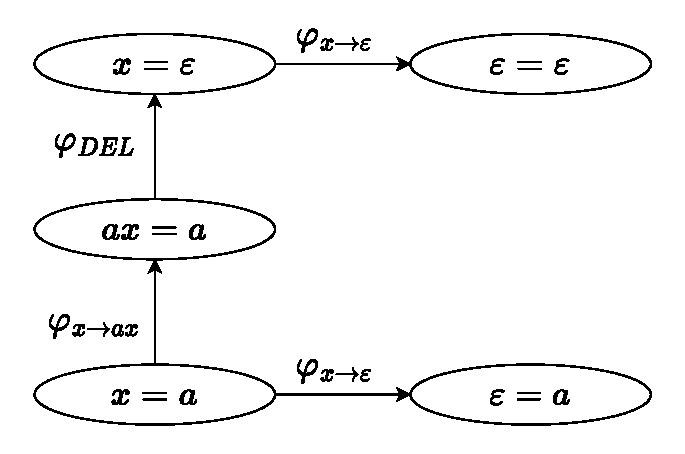
\includegraphics[]{images/x_a.pdf}
}
\caption{Graph for the satisfiable word equation $x = a$}
\label{fig:nielsen-graph-sat}
\end{center}
\end{figure}

Let us consider the simple and satisfiable word equation $x = a$. Figure \ref{fig:nielsen-graph-sat} shows the graph of the rewrites. We start at the bottom left with $x = a$. The equation can be rewritten, either by deleting $x$ and thus rewriting the equation by $\varphi_{x \rightarrow \varepsilon}$ (case \ref{def:nt_xe}), or by assuming that $a$ must be a prefix of $x$, triggering the rewrite $\varphi_{x \rightarrow ax}$ (case \ref{def:nt_xa}). In the latter case we arrive at the equation $ax = a$. We delete the prefix $a$ from both sides (case \ref{def:nt_aa}), arriving at $x = \varepsilon$. By deleting $x$ (case \ref{def:nt_xe}), we reach $\varepsilon = \varepsilon$. We reach $\varepsilon = \varepsilon$ from $x = a$ via the directed path characterized by the chain of rewrites $\varphi = \varphi_{x \rightarrow ax} \circ' \varphi_{DEL} \circ' \varphi_{x \rightarrow \varepsilon}$, because $\varphi(x) = \varepsilon = \varphi(a)$. We say $x = a$ is satisfiable with the solution $\varphi$.

\begin{figure}[H]
\begin{center}
\resizebox{0.6 \textwidth}{!}{
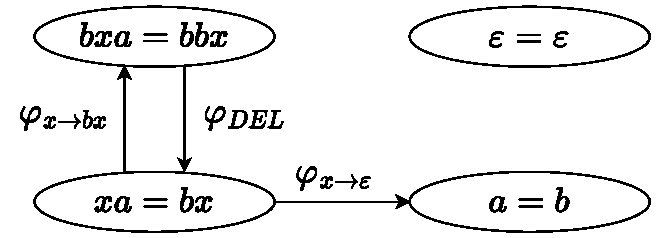
\includegraphics[]{images/xa_bx.pdf}
}
\caption{Graph for the unsatisfiable word equation $xa = bx$}
\label{fig:nielsen-graph-unsat}
\end{center}
\end{figure}

Let us now consider the case of an unsatisfiable equation: $xa = bx$ (figure \ref{fig:nielsen-graph-unsat}). We start at the bottom left and try to reach the top right node $\varepsilon = \varepsilon$. Again, we can either delete $x$ arriving at the dead end $a = b$, or we assume that $x$ has the prefix $b$. In this case we reach the equation $bxa = bbx$. We delete the shared prefix $b$ from both sides of the equation, bringing us back to $xa = bx$. No other rewrite rule applies. We cannot reach $\varepsilon = \varepsilon$. Therefore, the equation $xa = bx$ is unsatisfiable.

We reduced the satisfiability of word equations to a graph reachability problem. We can solve the reachability problem with any graph discovery algorithm. This includes depth-first search (DFS) and breadth-first search (BFS).
Interestingly, this also includes Dijkstra's \cite{dijkstra} algorithm for finding the shortest path. It generalizes BFS with a cost function. This cost function could be a heuristic, ranking each word equation by how promising it is to be reducible to $\varepsilon = \varepsilon$. Given a good cost function, Dijkstra could solve satisfiable equations faster than BFS. Note, however, that unsatisfiable equations would still take as long as with BFS, because Dijkstra's algorithm still has to perform an exhaustive graph search, if it cannot find a path. While this is an interesting idea, in this work we will not focus on finding heuristics.

To answer the question of satisfiability, we just need to find out whether some path of rewrites from $\alpha = \beta$ to $\varepsilon = \varepsilon$ exists. If we are interested in finding a satisfying variable assignment, we can backtrack over such a path. If we are interested in finding all assignments, we backtrack over all such paths.

Day et al. \cite{manea-nielsen} proved that the satisfiability problem for regular word equations is in NP and that for quadratic word equations the algorithm terminates in finite time.

This algorithm only works for unconstrained variables. In the next section we will have a look at regular expressions and how we can use them to constrain variables.

\section{Regular Expressions}
A regular expression $p$ over the alphabet $\Sigma$ describes a specific subset of $\Sigma^*$.
We use $L(p)$ to describe the set of words that are described by $p$. \cite{brzozowski}

We recursively define regular expressions to be either one of the base cases
\begin{enumerate}
    \item A symbol $a \in \Sigma$. $L(a) = \{a\}$
    \item The empty regex $\lambda$ that only matches the empty string $\varepsilon$. $L(\lambda) =            \{\varepsilon\}$
    \item The never matching regex $\emptyset$ that matches no string. $L(\emptyset) = \{\}$. This will later prove useful to model error states.
\end{enumerate}

Let $p, q$ be regular expressions over $\Sigma$. We now add the following recursive definitions to also be regular expressions

\begin{enumerate}
    \setcounter{enumi}{3}
    \item The concatenation $pq$. This matches all words $ww'$ where $w \in L(p), w' \in L(q) $
    \item The iteration $p*$. This regex matches zero or more occurrences of $p$. $L(p*) = L(\lambda) \cup L(p) \cup L(pp) \cup ...$
    \item The negation $p'$. This matches precicely when $p$ does not match. $L(p') = \Sigma^* \setminus L(p)$
    \item The conjunction $p\:\&\:q$. $L(p\:\&\:q) = L(p) \cap L(q)$
    \item The disjunction $p\:|\:q$. $L(p\:|\:q) = L(p) \cup L(q)$
\end{enumerate}

We denote the set of all regular expressions over $\Sigma$ as $R(\Sigma)$.


\subsection{Brzozowski Derivatives}
In his 1964 work, Brzozowski \cite{brzozowski} introduced a methodology for regular expression matching that does not construct an intermediary automaton. For this he defined a notion of \textit{derivatives} of a regular expression. The derivative of a regular expression $p$ respective to the symbol $a$ is the remainder of $p$ after successfully matching the first character $a$. Let us consider $a \in \Sigma, w \in \Sigma^*, p \in R(\Sigma)$. We define the derivative $D_ap$ in a way s.t. $aw \in L(p) \Leftrightarrow w \in L(D_ap)$.

Take for example the string $ab$ and the regex $a(b|c)$. To decide whether $ab \in a(b|c)$, we take the prefix of $ab$, i.e. $a$ and then calculate the derivative $D_a(a(b|c)) = b|c$. We reduced the matching problem $ab \in a(b|c)$ to $b \in b|c$. Now, we take the derivative $D_b(b|c) = \lambda|\emptyset$. We now reduced our problem to $\varepsilon \in \lambda|\emptyset$. Note that $\varepsilon \in L(\lambda) \cup L(\emptyset)$. Therefore, $ab \in a(b|c)$.

We always solve the matching problem by deriving character-by-character and then deciding whether the remaining regular expression matches $\varepsilon$:
Let $w = w_1w_2...w_n \in \Sigma^*$, then $w \in p \Leftrightarrow \varepsilon \in D_{w_n}(...(D_{w_2}(D_{w_1}p)))$. Thus, we only need a method of determining whether a regex $p$ is nullable, i.e. whether $\varepsilon \in p$. For this we define the nullability function $\nu: R(\Sigma) \rightarrow \{false, true\}$ with $\nu(p) \Leftrightarrow \varepsilon \in p$.

\[
\begin{tabular}{c c c}
    $\nu(\lambda)$ & $=$ & $true$ \\
    $\nu(\emptyset)$ & $=$ & $false$ \\
    $\nu(a)$ & $=$ & $false$ \\
    $\nu(pq)$ & $=$ & $\nu(p) \land \nu(q)$ \\
    $\nu(p*)$ & $=$ & $true$ \\
    $\nu(p')$ & $=$ & $\neg \nu(p)$ \\
    $\nu(p\:\&\:q)$ & $=$ & $\nu(p) \land \nu(q)$ \\
    $\nu(p\:|\:q)$ & $=$ & $\nu(p) \lor \nu(q)$ \\
\end{tabular}
\]

We can now define $D_ap$ as

\[
\begin{tabular}{c c l}
    $D_aa$ & $=$ & $\lambda$ \\
    $D_ab$ & $=$ & $\emptyset$ \\
    $D_a\lambda$ & $=$ & $\emptyset$ \\
    $D_a\emptyset$ & $=$ & $\emptyset$ \\

    $D_a(pq)$ & $=$ & $
    \left\{
	\begin{array}{ll}
		(D_ap)q\:|\:D_aq  & \mbox{if } \nu(p) \\
		(D_ap)q & \mbox{if } \neg \nu(p)
	\end{array}
    \right.
    $ \\
    
    $D_a(p*)$ & $=$ & $(D_ap)p*$ \\
    $D_a(p')$ & $=$ & $(D_ap)'$ \\
    $D_a(p\:\&\:q)$ & $=$ & $D_ap\:\&\:D_aq$ \\
    $D_a(p\:|\:q)$ & $=$ & $D_ap\:|\:D_aq$ \\
\end{tabular}
\]

Brzozowski also presented an algorithm to construct a DFA from a regular expression.
Brzozowski's notion of derivatives inspired an entire field of research and regex theories. In the following sections we will touch on two of these.

\subsection{Antimirov Derivatives}
In his 1995 work, Antimirov \cite{antimirov} introduced the notion of \textit{partial derivatives}. Just like Brzozowski's derivatives can be used to construct a DFA, Antimirov's partial derivatives can be used to construct an NFA. Antimirov does this by defining the partial derivative of $p$ respective to $a$ as $\partial_a : R(\Sigma) \rightarrow 2^{R(\Sigma)}$ as opposed to Brzozowski's $D_a : R(\Sigma) \rightarrow R(\Sigma)$. Antimirov also presents an algorithm for constructing a DFA that is more compact than Brzozowki's. 

\subsection{Transition Regexes}
Stanford et al. \cite{transition-regex} present the notion of \textit{symbolic derivatives}. Instead of operating on a regex, they return functions that later evaluate to regexes. By doing this, they delay branching and decision making for as long as possible. In their benchmarks they outperform Brzozowski derivatives and perform especially well on regular expressions with logical branches ($\&$ and $|$).

Both of these approaches are complete regex theories and can be used for regex matching. In this work, to keep it simple, we will only focus on the classic Brzozowski derivatives. In the next chapter, we will describe how to incorporate them into the Nielsen transformation.
    \chapter{Approach} \label{ch_approach}
The previous chapter introduced the Nielsen transformation, a prefix-based method to solve the satisfiability problem for unconstrained word equations, and Brzozowski's regex derivatives, a prefix-based method for regex matching. In this chapter, we present our approach of bringing both methods together, effectively extending the Nielsen transformation with regex derivatives to solve the satisfiability problem for regex-constrained word equations.

We now restrict the variables $x \in X$ by adding constraints $c(x) \in R(\Sigma)$.
An assignment $\assignment{\cdot}$ must satisfy these constraints. In other words, $\assignment{x} \in c(x)$ for all $x$.
This approach can handle unconstrained variables as well: For any unconstrained variable $x$, set $c(x)$ to be the catch-all regex $\emptyset'$ with $L(\emptyset') = \Sigma^* \setminus L(\emptyset) = \Sigma^*$.

Variables are now selected over (usually strict) subsets of $\Sigma^*$. This has severe consequences, as questions like "can $x$ be empty?", "is there a solution for $x$?" or "can $y$ be a prefix of $x$?" suddenly become non-trivial.

\section{Algorithm} \label{s_algorithm}
We modify Nielsen's algorithm to also cover regex-constrained variables. While some rewrite rules stay the same (i.e. if both sides start with a terminal symbol), a few rules change when moving from unconstrained to regex-constrained variables. This is because unconstrained variables are always \textit{satisfiable} (i.e. a solution exists) and \textit{nullable} (i.e. can be equal to $\varepsilon$), while for constrained variables we now have to add checks. In the sections \ref{ss_nullability} - \ref{ss_y_prefix_x}, we therefore take into account the ways in which constrained variables differ from unconstrained variables. In section \ref{ss_rnt}, we bring them together and present our modified version of the Nielsen transformation.

\subsection{Nullability} \label{ss_nullability}
While unconstrained variables, selected from $\Sigma^*$, are always \textit{nullable}, i.e. they can be empty, this does not hold for regex-constrained variables. 
Consider $x, c(x) = a\:|\:b$. Then $x$ is not nullable, because $\varepsilon \not\in c(x)$. Thus, no assignment $\assignment{\cdot}$ exists with $\assignment{x} = \varepsilon$. We need to take this into account because case \ref{def:nt_xe} of the Nielsen transformation deletes variables without checking for nullability first.


\subsection {Satisfiability}
Unconstrained variables always have some solution within $\Sigma^*$. Constrained variables on the other hand can have \textit{unsatisfiable} constraints. Take for example $x, c(x) = a\&b$. Then, there exists no assignment $\assignment{\cdot}$ with $\assignment{x} \in c(x)$, because $L(c(x)) = L(a) \cap L(b) = \{a\} \cap \{b\} = \{\}$. This breaks the current setup of the Nielsen transformation: Until now we always assumed that whenever we encounter a variable, there exists some value it can take. We need to take into account, that whenever we work with a variable, we have to check it for satisfiability first. This applies to the cases \ref{def:nt_xe} - \ref{def:nt_xy}.

We introduce the satisfiability function $\sigma: R(\Sigma) \rightarrow \{false, true\}$ with $\sigma(p) \Leftrightarrow L(p) \neq \{\}$.

\[
\begin{tabular}{c c c}
    $\sigma(\emptyset)$ & $=$ & $false$ \\
    $\sigma(\lambda)$ & $=$ & $true$ \\
    $\sigma(a)$ & $=$ & $true$ \\
    $\sigma(pq)$ & $=$ & $\sigma(p) \land \sigma(q)$ \\
    $\sigma(p*)$ & $=$ & $true$ \\
    $\sigma(p')$ & $=$ & $unknown$ \\
    $\sigma(p\:\&\:q)$ & $=$ & $\sigma(p) \land \sigma(q)$ \\
    $\sigma(p\:|\:q)$ & $=$ & $ \sigma(p) \lor \sigma(q)$ \\
\end{tabular}
\]

For $\sigma(p')$ we cannot determine the satisfiability. Consider the satisfiable regex $a|b$. Its negation $(a|b)'$ is satisfiable, because $aa \in (a|b)'$. Now consider the unsatisfiable regex $a\&b$. Again, its negation $(a\&b)'$ is satisfiable, because $a \in (a\&b)'$. So for these two regular expressions -- one satisfiable, the other unsatisfiable -- both negations are satisfiable. Still, let us consider $(a|b)*$ over the alphabet $\Sigma = \{a, b\}$. Then $L((a|b)*) = \Sigma^*$ and subsequently $L(((a|b)*)') = \{\}$, so the negation is unsatisfiable. The satisfiability of the negation $p'$ can therefore not be inferred from the satisfiability of $p$. To be safe, we assume that $p'$ is always satisfiable: $\sigma(p') = true$. Note, that this does not lead to incorrect results: A variable wrongly declared as satisfiable can only be deleted from the word equation later on, if it matches $\varepsilon$ and is therefore satisfiable.

\subsection{$a$ as a prefix of $x$}
If we now encounter case \ref{def:nt_xa} of the Nielsen transformation, i.e. $x\alpha = a\beta$, we assume that $x$ has the prefix $a$. For unconstrained variables this is always possible. For constrained variables we first need to find out if $x$ is allowed to start with $a$. In other words, we need to check that $\sigma(D_a(c(x))$. When rewriting with $\varphi_{x \rightarrow ax'}$, we also need to introduce the new constraint for $c(x') = D_a(c(x))$. If we recycle variable names, we update the constraint $c(x)$ instead.

\subsection{$y$ as a prefix of $x$} \label{ss_y_prefix_x}
For unconstrained variables, things are simpler: $y$ can always be a prefix of $x$.
For regex-constrained variables, it is not trivially possible to check whether one can be another variable's prefix because we have no simple way of finding out if $c(x)$ can begin with some $w \in L(c(y))$. We work around this issue by reformulating it. $y$ can be a prefix of $x$ if it is either empty (i.e. $y = \varepsilon$), or if $x = ax', y = ay'$ and $y'$ is a prefix of $x'$ for some $a \in \Sigma$. The case $y = \varepsilon$ can be safely disregarded because it is already covered in case \ref{def:nt_xe} of the Nielsen transformation. The other case just fixes a shared prefix $a$ for both variables and postpones the rest of the prefix problem for a later step of the Nielsen transformation.
For this to work, both $x$ and $y$ need to be allowed to start with $a$, in other words $\sigma(D_a(c(x))) \land \sigma(D_a(c(y)))$ needs to hold.

As we are interested in finding all $a \in \Sigma$ that fulfill this constraint, we define the prefix-function $\pi: R(\Sigma) \rightarrow 2^\Sigma, \pi(p) = \{a \in \Sigma\:|\:\sigma(D_ap)\}$ that can be algorithmically computed as follows:

\[
\begin{tabular}{c c l}
    $\pi(\lambda)$ & $=$ & $\{\}$ \\
    $\pi(\emptyset)$ & $=$ & $\{\}$ \\
    $\pi(a)$ & $=$ & $\{a\}$ \\
    
    $\pi(pq)$ & $=$ & $
        \left\{
    	\begin{array}{ll}
    		\pi(p) \cup \pi(q)  & \mbox{if } \nu(p) \\
    		\pi(p) & \mbox{if } \neg \nu(p)
    	\end{array}
        \right.
    $\\
    
    $\pi(p*)$ & $=$ & $\pi(p)$ \\
    $\pi(p')$ & $=$ & $unknown$ \\
    $\pi(p\:\&\:q)$ & $=$ & $\pi(p) \cap \pi(q)$ \\
    $\pi(p\:|\:q)$ & $=$ & $\pi(p) \cup \pi(q)$ \\
\end{tabular}
\]

For $\pi(p')$ we cannot determine the possible prefixes, so instead we say any symbol is possible and define $\pi(p') = \Sigma$.

For all $a \in \pi(c(x)) \cap \pi(c(y))$ (and those can be linearly many), we replace $y$ with $ay'$ by use of $\varphi_{y \rightarrow ay'}$ and introduce the new constraint $c(y') = D_a(c(y))$. It suffices to only cover $y = ay'$ and leave out $x = ax'$, because the resulting word equation $x\varphi_{y \rightarrow ay'}(\alpha) = ay'\varphi_{y \rightarrow ay'}(\beta)$ starts with $x$ and $a$ and thus triggers case \ref{def:nt_xa} immediately.

Note, that strictly speaking $\pi$ is not needed. Instead of iterating over $a \in \pi(c(x)) \cap \pi(c(y)) \subset \Sigma$, we could iterate over all $a \in \Sigma$ because unsatisfiable derivatives get filtered out later anyways. For large alphabets $\Sigma$ this comes with a blowup linear in $|\Sigma|$ for every application of case \ref{def:nt_xy}. This accumulates to an exponential blowup for repeated applications of case \ref{def:nt_xy}. We try to minimize this blowup by using $\pi$. This blowup does not exist in the unconstrained version of the Nielsen transformation. It is only introduced by our method of fixing shared prefixes $a$.

\subsection{Modified Algorithm} \label{ss_rnt}
To accommodate regex-constrained variables, we must modify the case analysis of the Nielsen transformation. We integrate the ideas from the previous chapters into the four cases \ref{def:nt_xe} - \ref{def:nt_xy} that deal with variable changes. The two non-terminal cases \ref{def:nt_aa} and \ref{def:nt_ab} stay the same. The updated case analysis looks like this:

Let $a, b \in \Sigma, a \neq b$ be two distinct terminals, $x, y \in X, x \neq y$ two distinct variables with constraints $c(x), c(y) \in R(\Sigma)$ and $\alpha, \beta \in (\Sigma \cup X)^*$ two (possibly equal) strings. Then for the Nielsen transformation, there are the following cases:

\begin{enumerate}
    \item \label{rnt_aa}
        Both sides start with the same terminal: $a\alpha = a\beta$. \\
        We can eliminate this terminal and reduce the equality problem to $\alpha =\beta$.
    
    \item \label{rnt_ab}
        Both sides start with a different terminal: $a\alpha = b\beta$ \\
        The strings cannot be equal because $a \neq b$.

    \item \label{rnt_xe}
        One side starts with a variable: $x\alpha = \beta$ \\
        If $x$ is satisfiable and nullable, i.e. if $\sigma(c(x)) \land \nu(c(x))$, we delete $x$ from the equation using $\varphi_{x \rightarrow \varepsilon}$.
        
        \begin{center}
        \begin{tabular}{r c l}
            $x\alpha$ & $=$ & $\beta$ \\    
            $\varphi_{x \rightarrow \varepsilon}(x\alpha)$ & $=$ & $\varphi_{x \rightarrow \varepsilon}(\beta)$ \\
            $\varphi_{x \rightarrow \varepsilon}(\alpha)$ & $=$ & $\varphi_{x \rightarrow \varepsilon}(\beta)$
        \end{tabular}
        \end{center}

    \item \label{rnt_xa}
        One side starts with a variable, and one starts with a terminal: $x\alpha = a\beta$\\
        If $x$ is satisfiable and if it can start with $a$, i.e. $\sigma(c(x)) \land \sigma(D_a(c(x)))$, we rewrite the equation using $\varphi_{x \rightarrow ax'}$ and we introduce the updated constraint $c(x') = D_a(c(x))$.
        
        \begin{center}
        \begin{tabular}{r c l}
            $x\alpha$ & $=$ & $a\beta$ \\
            $\varphi_{x \rightarrow ax'}(x\alpha)$ & $=$ & $\varphi_{x \rightarrow ax'}(a\beta)$ \\
            $ax'\varphi_{x \rightarrow ax'}(\alpha)$ & $=$ & $a\varphi_{x \rightarrow ax'}(\beta)$ \\
        \end{tabular}
        \end{center}

    \item \label{rnt_xx}
        Both sides start with the same variable: $x\alpha = x\beta$ \\
        If $x$ is satisfiable, i.e. if $\sigma(c(x))$, we delete the prefix $x$ from both sides of the equation leaving us with $\alpha = \beta$.
    
    \newpage
    
    \item \label{rnt_xy}
        Both strings start with different variables: $x\alpha = y\beta$ \\
        We fix a prefix for $y$. For all $a \in \pi(c(x)) \cap \pi(c(y))$, we rewrite using $\varphi_{y \rightarrow ay'}$.
        
        \begin{center}
        \begin{tabular}{r c l}
            $x\alpha$ & $=$ & $y\beta$ \\
            $\varphi_{y \rightarrow ay'}(x\alpha)$ & $=$ & $\varphi_{y \rightarrow ay'}(y\beta)$ \\
            $x\varphi_{y \rightarrow ay'}(\alpha)$ & $=$ & $ay'\varphi_{y \rightarrow ay'}(\beta)$ \\
        \end{tabular}
        \end{center}
\end{enumerate}

The rest of the algorithm stays unchanged: We try to find a directed path from $\alpha = \beta$ to $\varepsilon = \varepsilon$.

\section{Correctness}
\begin{theorem}
The algorithm formulated in \ref{s_algorithm} is correct. A solution for $\alpha = \beta$ exists, iff there is a path from $\alpha = \beta$ to $\varepsilon = \varepsilon$ in the graph of rewrites.
\end{theorem}

\begin{proof}
We will prove both sides of the equivalence separately.

Let $\varphi = \varphi_1 \circ' \varphi_2 \circ' ... \varphi_n$ be the path of rewrites so that $\varphi(\alpha) = \varepsilon = \varphi(\beta)$.

Now, ignore all prefix deletions $\varphi_{DEL}$ and group all rewrites by variable. For each variable $x$ we get $\varphi_x = \varphi_{x \rightarrow ax'} \circ' \varphi_{x' \rightarrow a'x''} \circ' ... \circ' \varphi_{x''' \rightarrow \varepsilon} = \varphi_{x \rightarrow aa'a''...}$. Note, that each $\varphi_x$ must end with $\varphi_{x''' \rightarrow \varepsilon}$, because otherwise $\varphi(\alpha) \neq \varepsilon$ or $
\varphi(\beta) \neq \varepsilon$. 
We define the assignment function $\assignment{x} = \varphi_x(x) = aa'a''...$ and the overall rewrite without prefix deletion $\Phi = \circ'_{x \in X} \varphi_x$ so that $\Phi(\alpha) = \Phi(\beta) \in \Sigma^*$. Then $\alpha = \beta$ holds with the assignment function $\assignment{\cdot}$.
Remember that rewrites of the form $\varphi_{x \rightarrow ax'}$ only exist if $\sigma(D_a(c(x)))$, and $\varphi_{x \rightarrow \varepsilon}$ only exists if $\nu(c(x))$, because otherwise our algorithm does not allow this rewrite. Therefore, $\nu(D_{a'''}(...(D_{a'}(D_a(c(x))))) \Leftrightarrow \varepsilon \in D_{a'''}(...(D_{a'}(D_a(c(x)))) \Leftrightarrow aa'...a''' \in c(x) \Leftrightarrow \assignment{x} \in c(x)$.
It follows that $\alpha = \beta$ has a solution $\assignment{\cdot}$ that satisfies the regex constraints.

Let us now consider the other direction. Let $\assignment{\cdot}$ be the assignment function of a solution for $\alpha = \beta$ that satisfies the regex constraints, i.e. $\assignment{x} \in c(x)$ for all variables $x$. We will now prove there exists a path $\varphi = \varphi_1 \circ' \varphi_2 \circ' ... \varphi_n$ so that $\varphi(\alpha) = \varepsilon = \varphi(\beta)$.

We make a case distinction:
\begin{enumerate}
    \item \label{proof_aa}
    $a\alpha = a\beta$: Both sides start with the same terminal symbol $a$.\\
    We rewrite the equation to $\alpha = \beta$ with $\varphi_{DEL}$ and repeat this case distinction.
    
    \item \label{proof_xe}
    $x\alpha = \beta$: One side starts with the variable $x$ and $\assignment{x} = \varepsilon$. Without loss of generality, we choose the left side.\\
    Note, that $\assignment{x} = \varepsilon$ implies $\nu(c(x))$. We rewrite with $\varphi_{x \rightarrow \varepsilon}$ and repeat this case distinction.
    
    \item \label{proof_xa}
    $x\alpha = a\beta$: One side starts with the variable $x$, the other side starts with the terminal symbol $a$, the assignment $\assignment{x}$ starts with $a$. Without loss of generality we chose the left side.\\
    We rewrite with $\varphi_{x \rightarrow ax'} \circ' \varphi_{DEL}$. Note, that here we have two rewrites because $\varphi_{x \rightarrow ax'}$ results in both sides of the equation starting with $a$. Therefore, we immediately follow up with $\varphi_{DEL}$. Afterwards, we repeat this case distinction.
    
    \item \label{proof_xy}
    $x\alpha = y\beta$: Both sides start with a variable ($x$ and $y$ may be the same), $\assignment{x}$ starts with $a$, $\assignment{y}$ starts with $a$. Note, that this implies $\sigma(D_a(c(x)))$ and $\sigma(D_a(c(y))$. We rewrite with $\varphi_{x \rightarrow ax'} \circ' \varphi_{y \rightarrow ay'} \circ' \varphi_{DEL}$ and repeat this case distinction.
    
    \item \label{proof_ee}
    $\varepsilon = \varepsilon$: The word equation has been fully reduced to $\varepsilon = \varepsilon$. We are done.
\end{enumerate}

This covers all possible cases. Cases like $a\alpha = b\beta$ for $a \neq b$ or $x\alpha = a\beta$ where $\assignment{x}$ does not start with $a$ need not be considered, because they are unsatisfiable and we assumed our word equation to be satisfiable. Furthermore, a rewrite done by the cases \ref{proof_aa} - \ref{proof_xy} always results in another equation that is still satisfiable.

To prove that we ultimately arrive at $\varepsilon = \varepsilon$, we must now only prove that each case moves us closer to $\varepsilon = \varepsilon$. We do this by showing that each case reduces the \textit{complexity} of the word equation.
We define the measure of complexity $||\cdot||$ to be $||\varepsilon|| = 0, ||a|| = 1, ||x|| = |\assignment{x}|+1, ||\alpha_1\alpha_2|| = ||\alpha_1|| + ||\alpha_2||$. We chose this particular definition of complexity solely so that every rewrite reduces the equation's complexity strictly monotonically. Also, this definition ensures that $||\alpha|| = 0 \Leftrightarrow \alpha = \varepsilon$. Let us use the short notation $||\varphi||$ for the change in complexity $\varphi$ achieves:
$||\varphi|| = ||\alpha\beta|| - ||\varphi(\alpha)\varphi(\beta)||$. Note, that $||\varphi_1 \circ' \varphi_2|| = ||\varphi_1|| + ||\varphi_2||$.

Case \ref{proof_aa} reduces the complexity of the word equation, because $||\varphi_{DEL}|| = -2$. Case \ref{proof_xe} also reduces the complexity of the word equation, because $||\varphi_{x \rightarrow \varepsilon}|| \in \{-1, -2\}$ depending on the number of occurrences of $x$. Let us now consider case \ref{proof_xa}. $||\varphi_{x \rightarrow ax'}|| = 0$, because $|\assignment{x'}| = |\assignment{x}| - 1$. Therefore, $||\varphi_{x \rightarrow ax'} \circ' \varphi_{DEL}|| = -2$.
Let us now consider the final case \ref{proof_xy}.
Again, $||\varphi_{x \rightarrow ax'} \circ' \varphi_{y \rightarrow ay'} \circ' \varphi_{DEL}|| = -2$. The only terminating case we can possibly choose is case \ref{proof_ee}. In other words, we only terminate for equations with complexity $0$. This entails that for a solution $\varphi$ with $\varphi(\alpha) = \varepsilon = \varphi(\beta)$ it always holds that $||\alpha\beta|| + ||\varphi|| = 0$.
Keep in mind that the cases \ref{proof_aa} - \ref{proof_xy} reduce the complexity by $1$ or $2$. Therefore, every word equation $\alpha = \beta$ terminates after $k$ iterations where $\frac{||\alpha\beta||}{2} \leq k \leq ||\alpha\beta||$.

\end{proof}

\newpage
\section{Complexity}

\begin{wrapfigure}{l}{0.5 \textwidth} \label{fig:hangup}
\begin{center}
\resizebox{0.4 \textwidth}{!}{
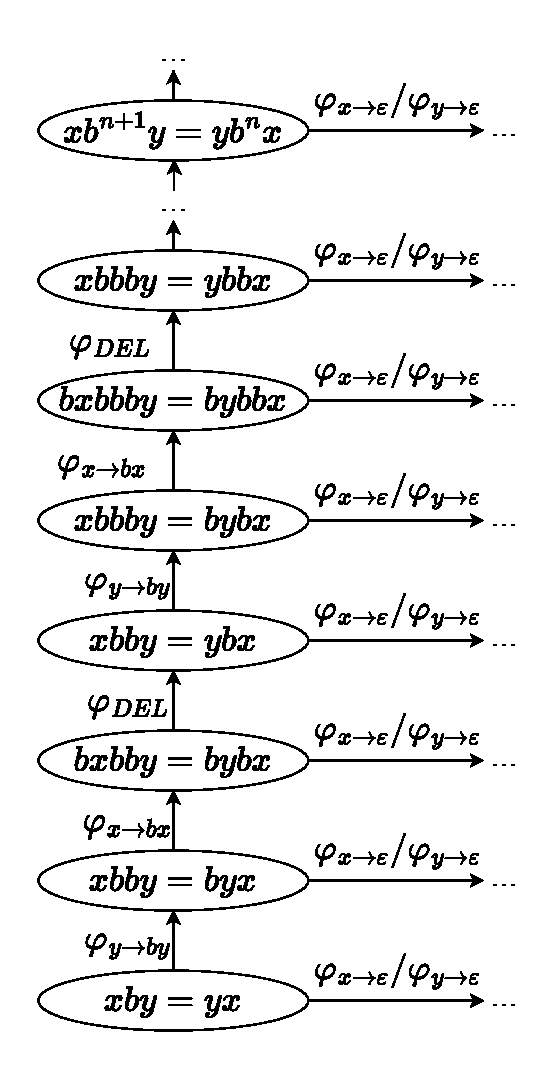
\includegraphics[]{images/xby_yx.pdf}
}
\caption{Graph for the non-terminating word equation $xby = yx, c(x) = (a|b)*, c(y) = b*$}
\label{fig:barplot-2-without-1}
\end{center}
\end{wrapfigure}
The algorithm does not terminate on all unsatisfiable word equations: Consider the equation
$xby = yx, c(x) = (a|b)*, c(y) = (b*)a$. We quickly see that rewriting it with $\varphi_{x \rightarrow \varepsilon}$ or $\varphi_{y \rightarrow \varepsilon}$ does not bring us towards $\varepsilon = \varepsilon$, because the resulting equations $xb = x$ and $by = y$ are dead ends.
Figure \ref{fig:hangup} shows the graph of rewrites. We start in the bottom left with $xby = yx$. We can either delete $x$ or $y$, by rewriting with $\varphi_{x \rightarrow \varepsilon}$ or $\varphi_{y \rightarrow \varepsilon}$, or we fix the shared prefix $b$. If we fix the shared prefix $b$, we trigger the chain of rewrites $\varphi_{y \rightarrow by} \circ' \varphi_{x \rightarrow bx} \circ' \varphi_{DEL}$. This leaves us with the new word equation $xbby = ybx$. The resulting equation again starts with $x$ on the left and $y$ on the right side. We can therefore again fix the prefix $b$. We see that repeating the rewrite chain $\varphi_{y \rightarrow by} \circ' \varphi_{x \rightarrow bx} \circ' \varphi_{DEL}$ for $n$ times gives us the equation $xb^{n+1}y = yb^nx$. We do not reach $\varepsilon = \varepsilon$ and are caught exploring an infinite graph. The algorithm does not terminate.

As we will see in the benchmarks later on, this is an extreme case and a very rare occurrence. Still, we are unable to guarantee that our algorithm terminates on unsatisfiable word equations.

~\\
For satisfiable word equations with a solution $\assignment{\cdot}$, the BFS can be bounded to terminate after $O(||\alpha\beta||)$ iterations. Each node can have $O(|\Sigma|)$ directed neighbors ($O(1)$ for the cases \ref{rnt_aa} - \ref{rnt_xx} and $O(|\Sigma|)$ for case \ref{rnt_xy}). This accumulates to $O(|\Sigma|^{||\alpha\beta||})$ many nodes visited before reaching $\varepsilon = \varepsilon$.

Note, that this does not mean that the satisfiability problem for regex-constrained word equations is undecidable, only that this particular algorithm cannot decide it. We could work around this by making use of regular expression \textit{quotients}.
Let $p, q \in R(\Sigma)$. We define the quotient $p/q$ to be the regular expression describing all words that match $p$ and have a prefix that matches $q$, without that prefix. In other words $L(p/q) = \{w_2\:|\:\exists\:w_1, w_2 \in \Sigma^*, w_1 \in L(q), w_1w_2 \in L(p)\}$. We observe that $D_ap = p/a$. If we can calculate the quotient $p/q$, we can solve the case \ref{rnt_xy} without having to fix a prefix $a$. Instead, when assuming $y$ to be a prefix of $x$, we rewrite with $\varphi_{x \rightarrow yx'}$ and introduce the new constraint $c(x') = c(x)/c(y)$.

\section{Extensibility}
The algorithm described in section \ref{s_algorithm} is agnostic to the regex theory at hand. It does not matter whether we use Brzozowski, Antimirov or transition regexes. The regex theory must only be \textit{derivative-based}, meaning it defines $D, \nu, \sigma, \pi$.

Simple length constraints of the form "$x$ must be of length $k$" can also be expressed as derivative-based constraints. Let $c(x) = k \in \mathbb{Z}$ stand for the constraint that $|\assignment{x}| = k$. Then the definitions

\[
\begin{tabular}{c c c}
    $D_ak$ & $=$ & $k-1$ \\
    $\nu(k)$ & $=$ & $k = 0$ \\
    $\sigma(k)$ & $=$ & $k \geq 0$ \\
    $\pi(k)$ & $=$ & $\Sigma$ \\
\end{tabular}
\]

allow us to integrate length constraints into the algorithm. In this work, although, we will only work with Brzozowski regex constraints.
    \chapter{Implementation} \label{ch_implementation}

We implement a string solver that uses the algorithm specified in chapter \ref{s_algorithm} in the programming language Haskell\footnote{https://github.com/meipp/nielsen-transformation}.
This chapter will introduce and document this solver. Readers who are not interested in technical-practical details may skip this chapter entirely.

\section{Haskell}
Haskell \cite{marlow2010haskell} is a purely functional, lazily-evaluated programming language with very expressive, declarative semantics. Purely functional means that Haskell data structures are immutable and that the language models side effects and IO as expressions. This makes optimization, verification and parallelization of Haskell programs fairly easy. Declarative means that instead of describing a process, we describe just a desired result and leave it to the runtime to evaluate our program. This makes it especially easy to write mathematical programs, as formulae can often be translated to Haskell in a very straightforward manner. Furthermore, Haskell also supports algebraic data types. The data type \texttt{Bool} can be defined in the following way:
\begin{minted}{haskell}
data Bool = False | True
\end{minted}
We introduce a new data type \texttt{Bool} whose values can either have the form \texttt{False} or \texttt{True}. For a more complex data type let us consider the data type \texttt{Either a b}. Its values encapsulate either a value of type \texttt{a} or a value of type \texttt{b}.
\begin{minted}{haskell}
data Either a b = Left a | Right b
\end{minted}
Here \texttt{a} and \texttt{b} are type variables. Values of the data type \texttt{Either String Int} for example can be constructed by writing \texttt{Left "hello"} or \texttt{Right 5}. For the above reasons, we chose Haskell as the language to implement our solver in.

\section{String Solvers}
String solvers are programs that solve string-related problems. As an input, they are given a \textit{test instance} consisting of a word equation or an instance for some other string problem. They then attempt to solve this problem in a given time interval. By convention they produce the outputs \textit{sat} if the problem is satisfiable, \textit{unsat} if unsatisfiable, \textit{unknown} if the algorithm in use cannot determine the problem's satisfiability, or \textit{timeout} if a predefined timeout has been reached.

\section{SMT-LIB}
In the string solving community, benchmarks and test instances usually come in a common file format: The SMT-LIB \cite{smtlib} format. SMT-LIB is a collaborative effort to maintain and publish a format that can be used by all solvers. SMT-LIB files all have a structure similar to this example:

\begin{minted}[xleftmargin=20pt, linenos]{lisp}
(declare-const x String)
(declare-const y String)
(assert (= (str.++ x "b") (str.++ "a" y "b")))
(assert (str.in_re x (re.++ (str.to_re "a") (re.* (str.to_re "b")))))
(assert (= (str.len y) 5))
(check-sat)
\end{minted}

In lines 1 and 2 we declare two variables \texttt{x} and \texttt{y}. As SMT-LIB also supports other data types, we must explicitly declare \texttt{x} and \texttt{y} to be string-valued variables. Lines 3 to 5 define all logical statements we \texttt{assert} to be true. Line 3 defines the word equation $\texttt{x}b = a\texttt{y}b$. Line 4 introduces the regex constraint $\texttt{x} \in ab*$. Line 5 introduces the length constraint $|\texttt{y}| = 5$. Line 6 instructs the solver to check for satisfiability. This word equation is satisfiable with exactly one solution: $\texttt{x} = abbbbb, \texttt{y} = bbbbb$.

\section{Architecture}

Our solver consists of four modules:
\begin{itemize}
    \item Algorithmic Core
    \item User definable Regex Theory
    \item SMT-LIB Interface
    \item Solver Frontend
\end{itemize}

\begin{figure}%[H]
\begin{center}
\includesvg{images/architecture.svg}
\caption{Architecture}
\label{fig:architecture}
\end{center}
\end{figure}

Figure \ref{fig:architecture} shows the architecture of our implementation. At its heart is the library with the generic implementation of our algorithm that can be extended by a user definable regex theory. The library can be used in Haskell programs or in most other languages, as Haskell's foreign function interface conforms to C-style function calls. The user defined regex theory is visualized as halfway part of the library and halfway on the outside because users can either use our implementation of Brzozowski's regex theory, or they can provide their own implementation. The algorithmic core is written to be completely agnostic to the regex theory used.

If the user instead decides to use our implementation as a full string solver, they have to call it on an SMT-LIB file. The solver frontend calls the SMT-LIB interface on the test instance. The SMT-LIB interface parses the instance to a regex-constrained word equation. The frontend then makes a library call to determine the satisfiability of the equation and outputs one of the results \textit{sat} or \textit{unsat}. The following sections give a detailed description of the four modules.

\subsection{User Definable Regex Theory}
The core of our approach does not care about the particular regex theory. The regex theory needs only define the functions $D, \nu, \sigma, \pi$. Therefore we keep it abstract and define a type class

\begin{minted}{haskell}
class RegexTheory r where
    derive :: Char -> r -> r
    nullable :: r -> Bool
    satisfiable :: r -> Bool
    possiblePrefixes :: r -> [Char]
\end{minted}

Every data type \texttt{r} that is an instance of the class \texttt{RegexTheory}, i.e. that implements the four functions \texttt{derive}, \texttt{nullable}, \texttt{satisfiable}, \texttt{possiblePrefixes}, can now be used to constrain variables. In chapters \ref{ch_foundations} and \ref{ch_approach}, we already defined $D, \nu, \sigma, \pi$ for Brzozowski derivatives. Our implementation of Brzozowski regexes instantiates the class \texttt{RegexTheory}.

\newpage

Note that $\sigma$ and $\pi$ are just optimizations and are technically speaking not needed in a minimal implementation. If we want to disregard them, we can provide the default implementations
\begin{minted}{haskell}
satisfiable r = True
possiblePrefixes r = sigma
\end{minted}
This has the effect that satisfiability checks for any regex return \texttt{True}. Unsatisfiable derivatives now do not get detected and discarded early. Still, this does not affect the correctness because unsatisfiable variables can never be deleted from the equation as they are not nullable ($\neg\sigma(p) \Rightarrow \neg\nu(p)$). Therefore, it is impossible to reduce a word equation that contains an unsatisfiable variable to $\varepsilon = \varepsilon$. The default implementation of the prefix function just returns the entire alphabet $\Sigma$. This also does not affect correctness because adding more symbols $a$ to calculate the derivative of, only results in more unsatisfiable regexes that again are ultimately not nullable.

\subsection{Algorithmic Core} \label{ss_backend}
The algorithmic core is the backend of our solver and is responsible for handling the core algorithm as defined in chapter \ref{s_algorithm}. We make the following definitions:

\begin{minted}{haskell}
data Terminal = Terminal Char
    deriving Eq

data Variable r = Variable Char r
    deriving Eq
\end{minted}

We introduce a new datatype \texttt{Terminal}. Each \texttt{Terminal} value is parameterized by only a  \texttt{Char} value. E.g. to represent the terminal symbol $a$, we write \texttt{Terminal 'a'}.
Similarly, we introduce \texttt{Variable r}, where \texttt{r} is a type parameter. Each variable is parameterized by a \texttt{Char}, i.e. its name, and by a regex value of type \texttt{r}. E.g. to represent the variable $x, c(x) = p$, we write \texttt{Variable 'x' p}. \texttt{deriving Eq} instructs the compiler to implement the canonical equality relation for our data types. I.e. \texttt{Terminal a == Terminal b} $\Leftrightarrow$ \texttt{a == b}.

For simplicity we introduce the following type aliases.

\begin{minted}{haskell}
type Symbol r = Either Terminal (Variable r)

type Sequence r = [Symbol r]

type Equation r = (Sequence r, Sequence r)
\end{minted}
A symbol is either a terminal or a variable. A sequence is a list of symbols. An equation is a tuple of two Sequences. We can now define the function
\begin{minted}{haskell}
nielsen :: RegexTheory r => Equation r -> Bool
\end{minted}

\texttt{nielsen} takes a word equation (constrained by some \texttt{RegexTheory r}) and returns \texttt{True} if it is satisfiable, \texttt{False} if it is unsatisfiable. As of now, we have implemented neither a timeout feature nor parallelization. Note, that we do not have to take care of \textit{unknown}s, because our algorithm can classify any input as either \textit{sat} or \textit{unsat}.

\subsection{SMT-LIB Interface}
The SMT-LIB interface parses \texttt{.smt} files and extracts word equations from them. Currently, we only support the subset of the SMT-LIB standard necessary to handle regex-constrained word equations, namely those functions required to define regex constraints, word equations as well as the instructions \texttt{not} and \texttt{assert}. We only support variables of type \texttt{String}. Functions like \texttt{str.len} are not supported.

Also, the parser is not agnostic to the regex theory and currently parses every regex constraint as a Brzozowski regex. This has the consequence that only the library is truly independent of the regex theory. For now, when using the string solver, we are bound to Brzozowski derivatives. One could solve this problem by adding a generic regex type
\begin{minted}{haskell}
data SmtLibRegex = Lambda
                 | Emptyset
                 | Symbol Char
                 | Concatenation SmtLibRegex SmtLibRegex
                 | Iteration SmtLibRegex
                 | Not SmtLibRegex
                 | And SmtLibRegex SmtLibRegex
                 | Or SmtLibRegex SmtLibRegex
\end{minted}
and the accompanying type class
\begin{minted}{haskell}
instance FromSmtLibRegex r where
    fromSmtLibRegex :: SmtLibRegex -> r
\end{minted}
The parser then parses regex constraints as values of the type \texttt{SmtLibRegex}. Those values can then get converted to our custom regex theories, as long as they provide an implementation for \texttt{fromSmtLibRegex}.

\newpage

\subsection{Solver Frontend}
The frontend handles the user interaction. It takes the file path of the \texttt{.smt} file as a command line argument, invokes the parser to parse a word equation and calls \texttt{nielsen} on it. It then outputs the result to \texttt{stdout}. The frontend can be expressed in the following pseudo code fragment:

\begin{minted}{bash}
filepath <- args[1]
equation <- SmtLibParser.parse(filepath)
if nielsen(equation)
    print "sat"
else
    print "unsat"
\end{minted}

where \texttt{args[1]} is the first command line argument, \texttt{SmtLibParser.parse} is a function that parses word equations with Brzozwski regex constraints from a file, and \texttt{nielsen} is the function introduced in section \ref{ss_backend}. Our implementation does not return \textit{unknown} on any instances and does not detect timeouts. For word equations that cannot be decided in finite time, the function \texttt{nielsen} does not terminate.
    \chapter{Benchmarks} \label{ch_benchmarks}
When comparing different approaches, the need arises to rank one against the other. For that, one usually employs benchmarks over benchmark sets. Benchmark sets are a collection of test instances used to evaluate the performance of algorithms. In the case of string solving, benchmark sets are usually in the SMT-LIB format and may consist of word equations, length constraints and regular expression constraints. These instances are usually either designed or curated to cover different aspects of the field. For example, one benchmark set may focus solely on small word equations with regex-constrained variables, while another may contain only very complex equations with length constraints.

This chapter focuses on the setup of our benchmarks. First, we explain the creation and makeup of the benchmark sets for our experiments. Then, we introduce the other string solvers we will compete against. Finally, we introduce the benchmarking framework ZaligVinder \cite{zaligvinder} that we will use to run the benchmarks.

\section{Building the Benchmark Sets}

First, let us have a look at how the benchmark sets are created.

\subsection{SMTQuery}
To automatically construct benchmark sets, we used the tool SMTQuery \cite{smtquery}.
SMTQuery allows running SQL-style queries on a predefined corpus of test instances.
The query
\begin{minted}{sql}
select Name from kaluza where isQuadratic
\end{minted}
lists the name of all test instances from the Kaluza \cite{benchmarkset-kaluza} benchmark set in which each variable occurs at most twice.

As a base corpus we use the ZaligVinder corpus \cite{zaligvinder}, which is a compilation of the following benchmark sets:

\begin{center}
\begin{tabular}{|l|r|}
\hline
Benchmark set & Instances \\
\hline
appscan \cite{benchmarkset-appscan-pisa} & 8 \\
automatark25 \cite{benchmarkset-automatark-stringfuzzregex} & 19979 \\
banditfuzz \cite{benchmarkset-banditfuzz} & 357 \\
cashewsuite \cite{benchmarkset-cashew} & 394 \\
joacosuite \cite{benchmarkset-joaco-stranger} & 94 \\
kaluza \cite{benchmarkset-kaluza} & 47284 \\
kauslersuite \cite{benchmarkset-kausler} & 120 \\
Leetcode \cite{benchmarkset-leetcode} & 2666 \\
light \cite{benchmarkset-light} & 100 \\
nornbenchmarks \cite{benchmarkset-norn} & 1027 \\
pisa \cite{benchmarkset-appscan-pisa} & 12 \\
PyEx\_All \cite{benchmarkset-pyex} & 25421 \\
slothtests \cite{benchmarkset-sloth} & 33 \\
strangersuite \cite{benchmarkset-joaco-stranger} & 4 \\
stringfuzz \cite{benchmarkset-stringfuzz} & 1065 \\
stringfuzzregexgenerated \cite{benchmarkset-automatark-stringfuzzregex} & 4170 \\
stringfuzzregextransformed \cite{benchmarkset-automatark-stringfuzzregex} & 10682 \\
woorpje \cite{woorpje} & 809 \\
z3\_regression \cite{benchmarkset-z3_regression} & 243 \\
\hline
$\Sigma$ & 114468 \\
\hline
\end{tabular}
\end{center}

This includes word equations -- quadratic or more complex --, regex matching, and other string problems. We will need to restrict the corpus when building our benchmark sets.

\subsection{benchmarkset-1}
Our approach solves word equations with regex-constrained variables. Thus, we are mainly interested in assessing its performance on test instances that follow this exact pattern. As the Nielsen transformation is only guaranteed to terminate on quadratic word equations \cite{manea-nielsen}, we will also restrict the benchmark set accordingly. Thus, we are interested only in \textbf{quadratic word equations with regex variable constraints}.
This leaves us with the SMT query

\begin{minted}{sql}
select Name from * where (hasWEQ and (isQuadratic and hasRegex))
\end{minted}

\newpage

This query selects all test instances over all benchmark sets for which the following restrictions hold:
\begin{enumerate}
    \item can be expressed as a word equation
    \item the word equation is quadratic
    \item the test instance contains at least one regex constraint
\end{enumerate}

This initially leaves us with 2859 out of 114468 instances. We still cannot process all of them. Therefore, we delete more files for the following reasons:

\begin{center}
\begin{tabular}{|l|r|}
    \hline
    Reason & Instances \\
    \hline
    declares Int variable & 25 \\
    declares Bool variable & 3 \\
    calls str.len & 422 \\
    calls str.to\_int & 85 \\
    contains multiple equations & 176 \\
    contains inequality & 1 \\
    \hline
    $\Sigma$ & 712 \\
    \hline
\end{tabular}
\end{center}

This concludes the construction of the benchmark set, leaving us with 2147 files.

\subsection{benchmarkset-2}
\texttt{benchmarkset-1} deals only with word equations where at least one variable has a regex constraint. We model unconstrained variables with the catch-all constraint $\emptyset'$. To assess the performance of our approach in a more general context, we drop the restriction that our variables must have regex constraints. We are left with a set of \textbf{quadratic word equations}. We construct the \texttt{benchmarkset-2} with the SMT query

\begin{minted}{sql}
select Name from * where (hasWEQ and isQuadratic)
\end{minted}

This leaves us with initially 26315 out of 114468 instances. Again, we clear the benchmark set of unprocessable instances:

\begin{center}
\begin{tabular}{|l|r|}
    \hline
    Reason & Instances \\
    \hline
    declares Int variable & 171 \\
    declares Bool variable & 21814 \\
    calls str.len & 516 \\
    calls str.to\_int & 85 \\
    calls to ite (if-then-else) & 51 \\
    contains multiple equations & 976 \\
    contains inequality & 157 \\
    \hline
    $\Sigma$ & 23770 \\
    \hline
\end{tabular}
\end{center}

This concludes the construction of the benchmark set with 2547 files.

We constructed this benchmark set with generality in mind, but we are limited by the fact that we only parse a subset of the SMT-LIB standard. In \texttt{benchmarkset-1} we reduced 2859 to 2147 files, a 24.9\% decrease. In \texttt{benchmarkset-2} on the other hand we have a decrease by 90.3\% going from 26315 files initially to just 2547 in the end.
We interpret this by assuming that there are not many test instances across the literature that contain unconstrained word equations. Most instances contain regex or length constraints. Thus, it is hard to find a truly general setting because a majority of the instances seems to be special cases.

\begin{figure}[H]
\begin{center}
\resizebox{0.5 \textwidth}{!}{
\includesvg[]{images/graphs/pie.svg}
}
\caption{Makeup of \texttt{benchmarkset-2}, divided in regex and non-regex word equations}
\label{fig:pie}
\end{center}
\end{figure}

Figure \ref{fig:pie} visualizes the makeup of \texttt{benchmarkset-2}. \texttt{benchmarkset-2} Is a superset of \texttt{benchmarkset-1}. It consists of the 2147 regex-constrained instances from \texttt{benchmarkset-1} and 400 more unconstrained instances.

\subsection{benchmarkset-2\:\textbackslash\:benchmarkset-1}
We constructed \texttt{benchmarkset-2} to assess our approach on a more general setting. Seeing that \texttt{benchmarkset-2} is bigger than \texttt{benchmarkset-1} by only 400 files (18.6\% increase), a quantitative analysis would be heavily biased towards instances with regex constraints, skewing our results. Therefore, we will also benchmark on the set difference \texttt{benchmarkset-2\:\textbackslash\:benchmarkset-1}, consisting only of quadratic, unconstrained instances that contain one word equation. This set should show the performance of our approach in a general setting that is not our algorithmic niche.

\newpage

\section{Other String Solvers}
This section discusses and introduces the string solvers we will benchmark against. We compare our approach to the state-of-the-art \cite{zaligvinder} solvers CVC4 \cite{cvc4}, Z3str3 \cite{z3str3} and Z3seq \cite{z3}. We also include the successor CVC5 \cite{cvc5}. Additionally, we compare to two other, less general solvers -- Woorpje \cite{woorpje} and Noodler \cite{noodler} -- because they share some interesting similarities with our approach.

\subsection{CVC4}
CVC4 \cite{cvc4}, the Cooperating Validity Checker 4, is a string/SMT solver that reduces its queries to SAT-formulae and solves them with a SAT-solver backend. It supports different \textit{Theories}, generates proofs and satisfying assignments. CVC4 supports highly parallelized execution. It is a collaborative effort between Stanford University and the University of Iowa.

CVC4 has been succeeded by CVC5 \cite{cvc5}. For the benchmarks we use version 1.8, which is the final release version of CVC4.

\subsection{CVC5}
CVC5 \cite{cvc5} is the successor to CVC4. CVC5 introduced a new proof engine, procedures for fixed-size bit vectors and non-linear arithmetic. Barbosa et al. \cite{cvc5} also claim that it outperforms CVC4 in terms of speed. As CVC4 has not been fully dethroned by its successor yet, we include both solvers for our benchmarks.

For our benchmarks we use version 1.0.3 of CVC5.

\subsection{Z3}
Z3 \cite{z3} is a general-purpose SMT solver published by Microsoft Research. It can handle quantifier-free as well as quantified formulae. Z3 cannot generate proofs, but it can generate models of satisfying assignments. Z3 contains multiple sub-solvers, called \textit{tactics}.

For our benchmarks we use version 4.8.10 of Z3. We benchmark against the following two state-of-the-art tactics.

\subsubsection{Z3seq}
Z3seq \cite{z3} is a tactic that processes strings in a prefix-based manner. Similar to our approach, Z3seq uses regex derivatives to check regex constraints. It differs from our approach in that it checks constraints and equations separately.

\subsubsection{Z3str3}
Z3str3 \cite{z3str3} is a solver tactic for Z3 that introduces a technique labeled \textit{theory-aware branching}, which extends Z3's branching heuristics allowing to pass information to the internal SAT-solver. Berzish et al. \cite{z3str3} claim, this technique improves the search step in Z3's solving engine, allowing for better performance.

\subsection{Woorpje}
The Woorpje string solver \cite{woorpje} specializes on word equations where every variable has an upper length bound, guessing unknown lengths. It reduces the bounded word equation to a SAT problem and solves it via the Glucose SAT solver \cite{glucose}. Woorpje also supports regex constraints and offers different solving strategies. More interestingly, Woorpje has one strategy that uses the Nielsen transformation, although Day et al. \cite{woorpje} refer to it as \textit{Levi's lemma}. As they use the traditional Nielsen transformation, this strategy only works for word equations without regex constraints. We will therefore use it only for benchmarking on \texttt{benchmarkset-2\:\textbackslash\:benchmarkset-1}. In the benchmarks, we will refer to Woorpje with the general strategy as \texttt{woorpje}, and to Woorpje with Levi's lemma as a strategy as \texttt{woorpje-levi}. This strategy is interesting because we can benchmark against a string solver that uses the same approach as ours.

In our benchmarks we use the release \texttt{spin22} of Woorpje.

\subsection{Noodler}
Noodler \cite{noodler} is the only string solver we are aware of that solves the word equation and the regex constraints together. Blahoudek et al. do this by representing each variable by an automaton and modeling the equation as concatenations of these automata.

As Noodler is not versionated, we used the commit \texttt{f752e79}\footnote{https://github.com/vhavlena/Noodler/commit/f752e79eb9c0cded7e7e1bf73476c3b1ef1f25b1} in our benchmarks.

This concludes the setup for our benchmarks. Figure \ref{fig:feature-matrix} gives a compact overview of the different string solvers we will use. Our solver is listed at the bottom as \texttt{nielsen-transformation}. We use version 0.1.0 of our solver\footnote{https://github.com/meipp/nielsen-transformation/releases/tag/0.1.0}.

\begin{figure}[H]
\begin{center}
\begin{tabular}{|c|c|c|c|c|}
    \hline
    Solver & Version & State of the art & Can solve regex & Combined solving \\
    \hline
    CVC4                   &    1.8 & \cellcolor{green!25}\cmark & \cellcolor{green!25}\cmark &
    \cellcolor{red!25}\xmark \\
    \hline
    CVC5                   &  1.0.3 & \cellcolor{green!25}\cmark & \cellcolor{green!25}\cmark &
    \cellcolor{red!25}\xmark \\
    \hline
    Z3Seq                  & 4.8.10 & \cellcolor{green!25}\cmark & \cellcolor{green!25}\cmark &
    \cellcolor{red!25}\xmark \\
    \hline
    Z3str3                 & 4.8.10 & \cellcolor{green!25}\cmark & \cellcolor{green!25}\cmark &
    \cellcolor{red!25}\xmark \\
    \hline
    woorpje                & spin22 &   \cellcolor{red!25}\xmark & \cellcolor{green!25}\cmark &
    \cellcolor{red!25}\xmark \\
    \hline
    woorpje-levi           & spin22 &   \cellcolor{red!25}\xmark &   \cellcolor{red!25}\xmark &
    \cellcolor{red!25}\xmark \\
    \hline
    noodler                & f752e79 &   \cellcolor{red!25}\xmark & \cellcolor{green!25}\cmark &
    \cellcolor{green!25}\cmark \\
    \hline
    nielsen-transformation &  0.1.0 &   \cellcolor{red!25}\xmark & \cellcolor{green!25}\cmark &
    \cellcolor{green!25}\cmark \\
    \hline
\end{tabular}
\caption{Comparison of previously introduced solvers. \textit{Combined solving} means that the solver solves the constraints and the word equation in a combined manner}
\label{fig:feature-matrix}
\end{center}
\end{figure}

\section{ZaligVinder}
To run the benchmarks we use the benchmarking framework ZaligVinder \cite{zaligvinder}. ZaligVinder brings benchmark sets and string solvers together on a shared platform. We configure it with test instances from our benchmark sets. For each solver, a shell command has to be registered that gets invoked on each test instance. ZaligVinder then counts all classifications. In case a solver does not terminate, ZaligVinder will count it as a timeout. Afterwards ZaligVinder produces tables for the measurements, in the format of appendix \ref{appendix_benchmarks}.
    \chapter{Results} \label{ch_results}
In this chapter, we present the findings of our benchmarks and a subsequent analysis. We ran the benchmarks on a system with an Intel i7-7500U CPU with four cores (2.70GHz base frequency, 3.50GHz Intel Turbo Boost) and 16GB of DDR4 memory. The complete results can be found in appendix \ref{appendix_benchmarks}. We used this\footnote{https://github.com/meipp/zaligvinder/releases/tag/0.1.0} particular setup for the benchmarks.

CVC, Z3 and our solver worked fine. Woorpje and Noodler had some problems with the regex-constrained equations. For Woorpje those errors are linked to the policy of guessing lengths. Noodler -- we found -- could not read the many Unicode escape sequences in the SMT-LIB files. This influences the correctness but not the time performance: A solver that immediately exits with \textit{unknown} does not get a time penalty.

\section{Benchmarks}
In this section we will present the results of the benchmarks on our three benchmark sets. The next section will give an interpretation of the results.

\subsection{benchmarkset-1}

\begin{figure}%[H]
\resizebox{\textwidth}{!}{
\begin{tabular}{c|r|r|r|r|r|r|r}
Solver & Satis & NSatis & Unknown & Timeout & Errors & Total Time & Total Time w/o Timeout\\
\hline
CVC4 & 747 & 1400 & 0 & 0 & 0 & 240297 & 240297\\
CVC5 & 747 & 1400 & 0 & 0 & 0 & 247331 & 247331\\
Z3seq & 748 & 1398 & 0 & 1 & 55 & 865382 & 845382\\
Z3str3 & 748 & 1398 & 0 & 1 & 55 & 950974 & 930974\\
woorpje & 393 & 643 & 684 & 427 & 126 & 13319883 & 4779883\\
noodler & 243 & 824 & 637 & 443 & 0 & 27816800 & 18956584\\
nielsen-transformation & 747 & 1398 & 0 & 2 & 0 & 251808 & 211808\\
\end{tabular}
}
\caption{Benchmark over \texttt{benchmarkset-1}}
\label{fig:benchmark-1}
\end{figure}

Figure \ref{fig:benchmark-1} shows the results of the benchmark on \texttt{benchmarkset-1} in the output format of ZaligVinder. The column \textit{Satis}, \textit{NSatis}, \textit{Unknown} refer to the number of instances the solver classified as satisfiable, unsatisfiable and unknown respectively. Unknowns can be either produced when the solver outputs an explicit "unknown" or when the solver does not produce an explicit "sat" or "unsat", crashes or does not give intelligible output. \textit{Timeout} refers to the number of instances for which the solver did not terminate within 20 seconds. The column \textit{Errors} refers to the number of instances where the program crashed or error output occurred. Note that errors still get counted as satisfiable, unsatisfiable or unknown. \textit{Total Time} refers to the time (in milliseconds) each solver took to solve all instances combined -- including a penalty of 20 seconds per timeout. \textit{Total Time w/o Timeout} refers to the overall time without that penalty.

The state-of-the-art solvers CVC and Z3, solve all instances without \textit{unknown}s. The Z3 solvers timeout on one instance while both CVC solvers can solve all instances within the time limit. Aside from the timeout, Z3 and CVC differ on only one other instance, with CVC classifying 747 instances and Z3 classifying 748 as satisfiable.
The solvers Woorpje and Noodler perform poorly across all metrics. They do not reach similar classifications like CVC or Z3. They return many unknowns, timeout on relatively many instances and frequently produce errors. Ultimately, their running time is also significantly worse. While unknowns may be blamed on them not being able to read some instances, the timeouts cannot.
Our solver, \texttt{nielsen-transformation}, is very close to the state-of-the-art solvers. We reach comparable results with the same number of satisfiable classifications as CVC and only one more timeout than Z3. Most importantly, looking at the \textit{Total Time w/o Timeout}, we outperform Z3 by far and are also slightly faster than CVC.

\begin{figure}%[H]
\begin{center}
\resizebox{0.6 \textwidth}{!}{
\includesvg{images/graphs/bar-1.svg}
}
\caption{Comparison of CVC, Z3 and our solver on \texttt{benchmarkset-1} (lower is better). \texttt{nt} refers to our solver.}
\label{fig:barplot-1}
\end{center}
\end{figure}

\newpage

Figure \ref{fig:barplot-1} highlights the performance of our solver against CVC and Z3. The margin by which we outperform CVC is slim, but we are an order of magnitude faster than Z3.

\subsection{benchmarkset-2}

\begin{figure}%[H]
\resizebox{\textwidth}{!}{
\begin{tabular}{c|r|r|r|r|r|r|r}
Solver & Satis & NSatis & Unknown & Timeout & Errors & Total Time & Total Time w/o Timeout\\
\hline
CVC4 & 1055 & 1491 & 0 & 1 & 0 & 326543 & 306543\\
CVC5 & 1055 & 1491 & 0 & 1 & 0 & 354380 & 334380\\
Z3seq & 1045 & 1409 & 0 & 93 & 55 & 2908422 & 1048422\\
Z3str3 & 1057 & 1408 & 5 & 77 & 55 & 2571637 & 1031637\\
woorpje & 693 & 651 & 695 & 508 & 127 & 15410164 & 5250164\\
noodler & 544 & 888 & 665 & 450 & 0 & 32926399 & 23926181\\
nielsen-transformation & 1011 & 1453 & 0 & 83 & 0 & 2371652 & 711652\\
\end{tabular}
}
\caption{Benchmark over \texttt{benchmarkset-2}}
\label{fig:benchmark-2}
\end{figure}

Figure \ref{fig:benchmark-2} shows the benchmark on \texttt{benchmarkset-2}. This includes regex-constrained and unconstrained word equations.
We observe roughly the same patterns as in figure \ref{fig:benchmark-1}: CVC performs well with just one timeout. Woorpje and Noodler perform poorly again.
Z3 looks very different than before: It has a significantly higher number of timeouts with 93 and 77 timeouts for Z3seq and Z3str3 respectively. One interesting observation is that Z3seq and Z3str3 behave differently. Z3seq has 16 more timeouts and one more classification as unsatisfiable, while Z3str3 has 12 more classifications as satisfiable and five more unknowns. On one hand, Z3str3 seems to be better at avoiding timeouts than Z3seq. This could be an example of the \textit{Theory-aware branching} at work. On the other hand, Z3str3 returns unknown for instances it cannot solve, while this behavior is seemingly not implemented in Z3seq.
Our solver performs worse than CVC and roughly similar to Z3. It has 83 timeouts, placing it between Z3str3 and Z3seq. It solves less satisfiable word equations than Z3 (1011 vs. 1045/1057) but more unsatisfiable word equations (1453 vs. 1408/1409). This is interesting because our approach can only reach the result unsatisfiable after an exhaustive graph search, running the risk of timeout. In this regard, we perform better than Z3 because we have a higher number of classifications as unsatisfiable, while not showing a higher number of timeouts.
When comparing running times, our solver still outperforms Z3, Woorpje and Noodler but is notably slower than CVC.


\begin{figure}%[H]
\begin{center}
\resizebox{0.6 \textwidth}{!}{
\includesvg{images/graphs/bar-2.svg}
}
\caption{Comparison of CVC, Z3 and our solver on \texttt{benchmarkset-2} (lower is better). \texttt{nt} refers to our solver.}
\label{fig:barplot-2}
\end{center}
\end{figure}

Figure \ref{fig:barplot-2} shows the performance of our solver against CVC and Z3. It can be placed pretty much in the middle, outperforming Z3 by a notable margin but also getting clearly outperformed by CVC.

\newpage

\subsection{benchmarkset-2\:\textbackslash\:benchmarkset-1}

\begin{figure}%[H]
\resizebox{\textwidth}{!}{
\begin{tabular}{c|r|r|r|r|r|r|r}
Solver & Satis & NSatis & Unknown & Timeout & Errors & Total Time & Total Time w/o Timeout\\
\hline
CVC4 & 308 & 91 & 0 & 1 & 0 & 90983 & 70983\\
CVC5 & 308 & 91 & 0 & 1 & 0 & 110981 & 90981\\
Z3seq & 297 & 11 & 0 & 92 & 0 & 2085124 & 245124\\
Z3str3 & 309 & 10 & 5 & 76 & 0 & 1643121 & 123121\\
woorpje & 299 & 4 & 8 & 89 & 0 & 2464010 & 684010\\
woorpje-levis & 300 & 90 & 9 & 1 & 1 & 206817 & 186817\\
noodler & 281 & 20 & 19 & 80 & 0 & 5256067 & 3656067\\
nielsen-transformation & 264 & 54 & 0 & 82 & 0 & 2111959 & 471959\\
\end{tabular}
}
\caption{Benchmark over \texttt{benchmarkset-2\:\textbackslash\:benchmarkset-1}}
\label{fig:benchmark-2-without-1}
\end{figure}

Figure \ref{fig:benchmark-2-without-1} shows the benchmark on \texttt{benchmarkset-2\:\textbackslash\:benchmarkset-1}. CVC and Z3 behave roughly the same as they did in \ref{fig:benchmark-2}. \texttt{woorpje} reached a satisfactory number of classifications on satisfiable instances but classified almost none as unsatisfiable. Noodler and our approach are completely unsatisfactory. Still, \texttt{woorpje}, Noodler and our solver do not perform worse than Z3 in terms of timeouts. \texttt{woorpje-levis}, on the other hand, performed really well, outperforming Z3 in terms of time and approaching CVC in terms of correctness. It also outperforms \texttt{woorpje} by far.


\begin{figure}%[H]
\begin{center}
\resizebox{0.6 \textwidth}{!}{
\includesvg{images/graphs/bar-2-without-1.svg}
}
\caption{Comparison of CVC, Z3, woorpje-levi and our solver on \texttt{benchmarkset-2\:\textbackslash\:benchmarkset-1} (lower is better). \texttt{nt} refers to our solver.}
\label{fig:barplot-2-without-1}
\end{center}
\end{figure}

Figure \ref{fig:barplot-2-without-1} shows the performance of our solver against CVC, Z3 and \texttt{woorpje-levi}. It gets outperformed by all solvers. \texttt{woorpje-levi} is placed between Z3str3 and Z3seq, showing that the Nielsen transformation as a solving strategy is competitive with Z3.

\section{Interpretation}
The interpretation of our findings is very straightforward: We perform well on \texttt{benchmarkset-1}, averagely on \texttt{benchmarkset-2} and badly on \texttt{benchmarkset-2\:\textbackslash\:benchmarkset-1}. This can be directly linked to the composition of the benchmark sets.

\texttt{benchmarkset-1} fits perfectly to our problem description: Word equations with regex constraints. We solve these well and outperform every other string solver, even the highly optimized CVC solvers. This leads us to the conclusion that choosing a combined approach that solves both word equation and regex constraints at the same time gives us an edge over approaches that solve equations and constraints separately.

\texttt{benchmarkset-2} consists of mainly regex-constrained word equations and some unconstrained word equations. We immediately lose our edge over CVC. We still perform well enough to beat Z3, although this can be explained by the majority of the instances being regex-constrained. We outperform the other solvers. Still, it is notable that our approach loses its clear advantage over the other solvers as soon as we move out of our niche.

\texttt{benchmarkset-2\:\textbackslash\:benchmarkset-1} consists solely of unconstrained word equations. Our solver gets outperformed by the state-of-the-art solvers. This makes sense because our only advantage was the combination of regex constraints with the word equation. As soon as we lose the regex constraints, we lose all foundation we had for an advantage. Not only that but now our solver can only make use of the Nielsen transformation and has to compete with other solvers that can choose from a multitude of tactics which may include the Nielsen transformation. Subsequently, our solver performs significantly worse.

\texttt{woorpje-levis} -- being competitive with Z3 -- shows that the Nielsen transformation is viable for unconstrained word equations. It also shows that our implementation is not optimal in terms of running time. This is most likely due to Woorpje being more optimized on an instruction level. Also, we model unconstrained variables as $\emptyset'$ and unnecessarily calculate their derivative.

This concludes our findings. \texttt{woorpje-levis} shows that the Nielsen transformation is a valid tactic for solving unconstrained word equations. When combined with regex constraints in a combined approach, as shown by our reference implementation, the Nielsen transformation becomes a powerful tool outperforming even state-of-the-art solvers. Our approach was competitive inside of the specific niche of regex-constrained word equations. While it is not suitable as a general string solver, it could be used as a specialized tactic inside a portfolio solver.

    \chapter{Conclusion} \label{ch_conclusion}

We presented an algorithm to solve regex-constrained as well as unconstrained word equations and provided a reference implementation. We compiled and published three benchmark sets specialized for Nielsen-based approaches. Our implementation outperforms current state-of-the-art solvers on quadratic, regex-constrained word equations. We conclude that our approach is best applied as a tactic.

While this thesis provided an initial proof of concept showing the viability of our approach, much future work can still be done.

Firstly, our solver supports neither length constraints nor equation systems containing more than one equation. This means we are not compatible with the entire SMT-LIB standard and thus cannot compete in string solving competitions.

Secondly, this solver is currently implemented as a standalone solver. As explained earlier, it would make most sense to implement it as a solver tactic for either one of the state-of-the-art solvers or in a portfolio solver.

Lastly, one could extend the algorithm in multiple ways.
For once, we only implemented Brzozowski derivatives. One could instead implement transition regexes to see whether their claimed advantage \cite{transition-regex} also holds within our approach. Furthermore, we noted that Dijkstra's algorithm can be used when given a heuristic. One could try different heuristics ranking word equations in terms of prospected solvability.
Finally, we note that simple length constraints can also be expressed as derivative-based constraints. A future version of our solver could therefore possibly also handle length constraints.
One last drawback of our algorithm is that it is not guaranteed to terminate on some unsatisfiable equations. This problem can be solved by making use of regex quotients.

    %--- references ---
    \bibliographystyle{IEEEtran}
    \bibliography{content/references}
    \addcontentsline{toc}{chapter}{\bibname}

    %--- appendix ---
    \begin{appendix}
        \chapter{Benchmarks} \label{appendix_benchmarks}

This chapter shows the benchmark results as produced by ZaligVinder. ZaligVinder partitions the benchmark sets into subsets, so-called tracks. \texttt{benchmarkset-1} has the track \texttt{kaluza} which corresponds with the instances of \texttt{benchmarkset-1} originally from the Kaluza benchmark set. Because of ZaligVinder's naming conventions, we refer to \texttt{benchmarkset-2\:\textbackslash\:benchmarkset-1} as \texttt{benchmarkset-2-without-1}.

\section{benchmarkset-1}

Track: benchmarkset-1/joacosuite

\resizebox{\textwidth}{!}{
\begin{tabular}{c|r|r|r|r|r|r|r|r}
Solver & Satis & NSatis & Unknown & Timeout & Errors & SMT Solver Calls & Total Time & Total Time w/o Timeout \\
\hline
CVC4 & 2 & 0 & 0 & 0 & 0 & 2 & 459 & 459 \\
CVC5 & 2 & 0 & 0 & 0 & 0 & 2 & 563 & 563 \\
Z3seq & 2 & 0 & 0 & 0 & 4 & 2 & 563 & 563 \\
Z3str3 & 2 & 0 & 0 & 0 & 4 & 2 & 301 & 301 \\
woorpje & 0 & 0 & 2 & 0 & 0 & 2 & 194 & 194 \\
noodler & 0 & 0 & 2 & 0 & 0 & 2 & 2254 & 2254 \\
nielsen-transformation & 2 & 0 & 0 & 0 & 0 & 2 & 31 & 31 \\
\end{tabular}
}
~\\
Track: benchmarkset-1/kaluza

\resizebox{\textwidth}{!}{
\begin{tabular}{c|r|r|r|r|r|r|r|r}
Solver & Satis & NSatis & Unknown & Timeout & Errors & SMT Solver Calls & Total Time & Total Time w/o Timeout \\
CVC4 & 323 & 0 & 0 & 0 & 0 & 323 & 40137 & 40137 \\
CVC5 & 323 & 0 & 0 & 0 & 0 & 323 & 40894 & 40894 \\
Z3seq & 323 & 0 & 0 & 0 & 0 & 323 & 116686 & 116686 \\
Z3str3 & 323 & 0 & 0 & 0 & 0 & 323 & 122030 & 122030 \\
woorpje & 323 & 0 & 0 & 0 & 0 & 323 & 118300 & 118300 \\
noodler & 0 & 0 & 323 & 0 & 0 & 323 & 3477941 & 3477941 \\
nielsen-transformation & 323 & 0 & 0 & 0 & 0 & 323 & 29044 & 29044 \\
\end{tabular}
}

\newpage

Track: benchmarkset-1/slothtests

\resizebox{\textwidth}{!}{
\begin{tabular}{c|r|r|r|r|r|r|r|r}
Solver & Satis & NSatis & Unknown & Timeout & Errors & SMT Solver Calls & Total Time & Total Time w/o Timeout \\
\hline
CVC4 & 1 & 4 & 0 & 0 & 0 & 5 & 810 & 810 \\
CVC5 & 1 & 4 & 0 & 0 & 0 & 5 & 887 & 887 \\
Z3seq & 2 & 2 & 0 & 1 & 1 & 5 & 20889 & 889 \\
Z3str3 & 2 & 2 & 0 & 1 & 1 & 5 & 21017 & 1017 \\
woorpje & 3 & 0 & 1 & 1 & 2 & 5 & 23362 & 3362 \\
noodler & 1 & 1 & 3 & 0 & 0 & 5 & 15861 & 15861 \\
nielsen-transformation & 1 & 2 & 0 & 2 & 0 & 5 & 40207 & 207 \\
\end{tabular}
}
~\\
Track: benchmarkset-1/stringfuzzregextransformed

\resizebox{\textwidth}{!}{
\begin{tabular}{c|r|r|r|r|r|r|r|r}
Solver & Satis & NSatis & Unknown & Timeout & Errors & SMT Solver Calls & Total Time & Total Time w/o Timeout \\
\hline
CVC4 & 418 & 1392 & 0 & 0 & 0 & 1810 & 198491 & 198491 \\
CVC5 & 418 & 1392 & 0 & 0 & 0 & 1810 & 204621 & 204621 \\
Z3seq & 418 & 1392 & 0 & 0 & 50 & 1810 & 725639 & 725639 \\
Z3str3 & 418 & 1392 & 0 & 0 & 50 & 1810 & 806071 & 806071 \\
woorpje & 67 & 639 & 678 & 426 & 124 & 1810 & 13170095 & 4650095 \\
noodler & 239 & 820 & 308 & 443 & 0 & 1810 & 24299726 & 15439510 \\
nielsen-transformation & 418 & 1392 & 0 & 0 & 0 & 1810 & 182150 & 182150 \\
\end{tabular}
}
~\\
Track: benchmarkset-1/z3\_regression

\resizebox{\textwidth}{!}{
\begin{tabular}{c|r|r|r|r|r|r|r|r}
Solver & Satis & NSatis & Unknown & Timeout & Errors & SMT Solver Calls & Total Time & Total Time w/o Timeout \\
\hline
CVC4 & 3 & 4 & 0 & 0 & 0 & 7 & 400 & 400 \\
CVC5 & 3 & 4 & 0 & 0 & 0 & 7 & 366 & 366 \\
Z3seq & 3 & 4 & 0 & 0 & 0 & 7 & 1605 & 1605 \\
Z3str3 & 3 & 4 & 0 & 0 & 0 & 7 & 1555 & 1555 \\
woorpje & 0 & 4 & 3 & 0 & 0 & 7 & 7932 & 7932 \\
noodler & 3 & 3 & 1 & 0 & 0 & 7 & 21018 & 21018 \\
nielsen-transformation & 3 & 4 & 0 & 0 & 0 & 7 & 376 & 376 \\
\end{tabular}
}
~\\
Total

\resizebox{\textwidth}{!}{
\begin{tabular}{c|r|r|r|r|r|r|r|r}
Solver & Satis & NSatis & Unknown & Timeout & Errors & SMT Solver Calls & Total Time & Total Time w/o Timeout\\
\hline
CVC4 & 747 & 1400 & 0 & 0 & 0 & 2147 & 240297 & 240297\\
CVC5 & 747 & 1400 & 0 & 0 & 0 & 2147 & 247331 & 247331\\
Z3seq & 748 & 1398 & 0 & 1 & 55 & 2147 & 865382 & 845382\\
Z3str3 & 748 & 1398 & 0 & 1 & 55 & 2147 & 950974 & 930974\\
woorpje & 393 & 643 & 684 & 427 & 126 & 2147 & 13319883 & 4779883\\
noodler & 243 & 824 & 637 & 443 & 0 & 2147 & 27816800 & 18956584\\
nielsen-transformation & 747 & 1398 & 0 & 2 & 0 & 2147 & 251808 & 211808\\
\end{tabular}
}

Benchmark took 20 minutes, 5 seconds

\newpage

\section{benchmarkset-2}

Track: benchmarkset-2/cashewsuite

\resizebox{\textwidth}{!}{
\begin{tabular}{c|r|r|r|r|r|r|r|r}
Solver & Satis & NSatis & Unknown & Timeout & Errors & SMT Solver Calls & Total Time & Total Time w/o Timeout \\
\hline
CVC4 & 121 & 0 & 0 & 0 & 0 & 121 & 12706 & 12706 \\
CVC5 & 121 & 0 & 0 & 0 & 0 & 121 & 13384 & 13384 \\
Z3seq & 121 & 0 & 0 & 0 & 0 & 121 & 41413 & 41413 \\
Z3str3 & 121 & 0 & 0 & 0 & 0 & 121 & 42507 & 42507 \\
woorpje & 121 & 0 & 0 & 0 & 0 & 121 & 36453 & 36453 \\
noodler & 121 & 0 & 0 & 0 & 0 & 121 & 1219908 & 1219908 \\
nielsen-transformation & 121 & 0 & 0 & 0 & 0 & 121 & 11903 & 11903 \\
\end{tabular}
}
~\\
Track: benchmarkset-2/kaluza

\resizebox{\textwidth}{!}{
\begin{tabular}{c|r|r|r|r|r|r|r|r}
Solver & Satis & NSatis & Unknown & Timeout & Errors & SMT Solver Calls & Total Time & Total Time w/o Timeout \\
\hline
CVC4 & 323 & 0 & 0 & 0 & 0 & 323 & 38734 & 38734 \\
CVC5 & 323 & 0 & 0 & 0 & 0 & 323 & 41070 & 41070 \\
Z3seq & 323 & 0 & 0 & 0 & 0 & 323 & 115946 & 115946 \\
Z3str3 & 323 & 0 & 0 & 0 & 0 & 323 & 123330 & 123330 \\
woorpje & 323 & 0 & 0 & 0 & 0 & 323 & 121773 & 121773 \\
noodler & 0 & 0 & 323 & 0 & 0 & 323 & 3406691 & 3406691 \\
nielsen-transformation & 323 & 0 & 0 & 0 & 0 & 323 & 30998 & 30998 \\
\end{tabular}
}
~\\
Track: benchmarkset-2/slothtests

\resizebox{\textwidth}{!}{
\begin{tabular}{c|r|r|r|r|r|r|r|r}
Solver & Satis & NSatis & Unknown & Timeout & Errors & SMT Solver Calls & Total Time & Total Time w/o Timeout \\
\hline
CVC4 & 3 & 5 & 0 & 0 & 0 & 8 & 1234 & 1234 \\
CVC5 & 3 & 5 & 0 & 0 & 0 & 8 & 1407 & 1407 \\
Z3seq & 4 & 3 & 0 & 1 & 1 & 8 & 22224 & 2224 \\
Z3str3 & 4 & 3 & 0 & 1 & 1 & 8 & 22239 & 2239 \\
woorpje & 4 & 0 & 2 & 2 & 2 & 8 & 45100 & 5100 \\
noodler & 2 & 2 & 4 & 0 & 0 & 8 & 33160 & 33160 \\
nielsen-transformation & 3 & 3 & 0 & 2 & 0 & 8 & 40869 & 869 \\
\end{tabular}
}
~\\
Track: benchmarkset-2/stringfuzzregextransformed

\resizebox{\textwidth}{!}{
\begin{tabular}{c|r|r|r|r|r|r|r|r}
Solver & Satis & NSatis & Unknown & Timeout & Errors & SMT Solver Calls & Total Time & Total Time w/o Timeout \\
\hline
CVC4 & 418 & 1392 & 0 & 0 & 0 & 1810 & 195276 & 195276 \\
CVC5 & 418 & 1392 & 0 & 0 & 0 & 1810 & 201724 & 201724 \\
Z3seq & 418 & 1392 & 0 & 0 & 50 & 1810 & 695118 & 695118 \\
Z3str3 & 418 & 1392 & 0 & 0 & 50 & 1810 & 778418 & 778418 \\
woorpje & 67 & 643 & 681 & 419 & 125 & 1810 & 12886536 & 4506536 \\
noodler & 257 & 862 & 317 & 374 & 0 & 1810 & 23735000 & 16254782 \\
nielsen-transformation & 418 & 1392 & 0 & 0 & 0 & 1810 & 171385 & 171385 \\
\end{tabular}
}

Track: benchmarkset-2/woorpje

\resizebox{\textwidth}{!}{
\begin{tabular}{c|r|r|r|r|r|r|r|r}
Solver & Satis & NSatis & Unknown & Timeout & Errors & SMT Solver Calls & Total Time & Total Time w/o Timeout \\
\hline
CVC4 & 160 & 4 & 0 & 1 & 0 & 165 & 58997 & 38997 \\
CVC5 & 160 & 4 & 0 & 1 & 0 & 165 & 70517 & 50517 \\
Z3seq & 149 & 4 & 0 & 12 & 0 & 165 & 418467 & 178467 \\
Z3str3 & 161 & 4 & 0 & 0 & 0 & 165 & 68214 & 68214 \\
woorpje & 154 & 0 & 4 & 7 & 0 & 165 & 672842 & 532842 \\
noodler & 137 & 4 & 11 & 13 & 0 & 165 & 2692342 & 2432342 \\
nielsen-transformation & 116 & 3 & 0 & 46 & 0 & 165 & 1208948 & 288948 \\
\end{tabular}
}

\newpage

Track: benchmarkset-2/joacosuite

\resizebox{\textwidth}{!}{
\begin{tabular}{c|r|r|r|r|r|r|r|r}
Solver & Satis & NSatis & Unknown & Timeout & Errors & SMT Solver Calls & Total Time & Total Time w/o Timeout \\
\hline
CVC4 & 2 & 0 & 0 & 0 & 0 & 2 & 646 & 646 \\
CVC5 & 2 & 0 & 0 & 0 & 0 & 2 & 721 & 721 \\
Z3seq & 2 & 0 & 0 & 0 & 4 & 2 & 454 & 454 \\
Z3str3 & 2 & 0 & 0 & 0 & 4 & 2 & 435 & 435 \\
woorpje & 0 & 0 & 2 & 0 & 0 & 2 & 227 & 227 \\
noodler & 0 & 0 & 2 & 0 & 0 & 2 & 2300 & 2300 \\
nielsen-transformation & 2 & 0 & 0 & 0 & 0 & 2 & 72 & 72 \\
\end{tabular}
}
~\\
Track: benchmarkset-2/stringfuzz

\resizebox{\textwidth}{!}{
\begin{tabular}{c|r|r|r|r|r|r|r|r}
Solver & Satis & NSatis & Unknown & Timeout & Errors & SMT Solver Calls & Total Time & Total Time w/o Timeout \\
\hline
CVC4 & 0 & 80 & 0 & 0 & 0 & 80 & 13707 & 13707 \\
CVC5 & 0 & 80 & 0 & 0 & 0 & 80 & 17936 & 17936 \\
Z3seq & 0 & 0 & 0 & 80 & 0 & 80 & 1600000 & 0 \\
Z3str3 & 0 & 0 & 4 & 76 & 0 & 80 & 1521530 & 1530 \\
woorpje & 0 & 0 & 1 & 79 & 0 & 80 & 1580695 & 695 \\
noodler & 0 & 11 & 6 & 63 & 0 & 80 & 1559094 & 299094 \\
nielsen-transformation & 0 & 45 & 0 & 35 & 0 & 80 & 866514 & 166514 \\
\end{tabular}
}
~\\
Track: benchmarkset-2/z3\_regression

\resizebox{\textwidth}{!}{
\begin{tabular}{c|r|r|r|r|r|r|r|r}
Solver & Satis & NSatis & Unknown & Timeout & Errors & SMT Solver Calls & Total Time & Total Time w/o Timeout \\
\hline
CVC4 & 28 & 10 & 0 & 0 & 0 & 38 & 5243 & 5243 \\
CVC5 & 28 & 10 & 0 & 0 & 0 & 38 & 7621 & 7621 \\
Z3seq & 28 & 10 & 0 & 0 & 0 & 38 & 14800 & 14800 \\
Z3str3 & 28 & 9 & 1 & 0 & 0 & 38 & 14964 & 14964 \\
woorpje & 24 & 8 & 5 & 1 & 0 & 38 & 66538 & 46538 \\
noodler & 27 & 9 & 2 & 0 & 0 & 38 & 277904 & 277904 \\
nielsen-transformation & 28 & 10 & 0 & 0 & 0 & 38 & 40963 & 40963 \\
\end{tabular}
}
~\\
Total

\resizebox{\textwidth}{!}{
\begin{tabular}{c|r|r|r|r|r|r|r|r}
Solver & Satis & NSatis & Unknown & Timeout & Errors & SMT Solver Calls & Total Time & Total Time w/o Timeout\\
\hline
CVC4 & 1055 & 1491 & 0 & 1 & 0 & 2547 & 326543 & 306543\\
CVC5 & 1055 & 1491 & 0 & 1 & 0 & 2547 & 354380 & 334380\\
Z3seq & 1045 & 1409 & 0 & 93 & 55 & 2547 & 2908422 & 1048422\\
Z3str3 & 1057 & 1408 & 5 & 77 & 55 & 2547 & 2571637 & 1031637\\
woorpje & 693 & 651 & 695 & 508 & 127 & 2547 & 15410164 & 5250164\\
noodler & 544 & 888 & 665 & 450 & 0 & 2547 & 32926399 & 23926181\\
nielsen-transformation & 1011 & 1453 & 0 & 83 & 0 & 2547 & 2371652 & 711652\\
\end{tabular}
}
~\\
Benchmark took 26 minutes, 25 seconds

\newpage

\section{benchmarkset-2\:\textbackslash\:benchmarkset-1}

Track: benchmarkset-2-without-1/cashewsuite

\resizebox{\textwidth}{!}{
\begin{tabular}{c|r|r|r|r|r|r|r|r}
Solver & Satis & NSatis & Unknown & Timeout & Errors & SMT Solver Calls & Total Time & Total Time w/o Timeout \\
\hline
CVC4 & 121 & 0 & 0 & 0 & 0 & 121 & 10697 & 10697 \\
CVC5 & 121 & 0 & 0 & 0 & 0 & 121 & 12488 & 12488 \\
Z3seq & 121 & 0 & 0 & 0 & 0 & 121 & 40995 & 40995 \\
Z3str3 & 121 & 0 & 0 & 0 & 0 & 121 & 40944 & 40944 \\
woorpje & 121 & 0 & 0 & 0 & 0 & 121 & 36876 & 36876 \\
woorpje-levis & 121 & 0 & 0 & 0 & 0 & 121 & 43058 & 43058 \\
noodler & 121 & 0 & 0 & 0 & 0 & 121 & 988793 & 988793 \\
nielsen-transformation & 121 & 0 & 0 & 0 & 0 & 121 & 9789 & 9789 \\
\end{tabular}
}
~\\
Track: benchmarkset-2-without-1/slothtests

\resizebox{\textwidth}{!}{
\begin{tabular}{c|r|r|r|r|r|r|r|r}
Solver & Satis & NSatis & Unknown & Timeout & Errors & SMT Solver Calls & Total Time & Total Time w/o Timeout \\
\hline
CVC4 & 2 & 1 & 0 & 0 & 0 & 3 & 60 & 60 \\
CVC5 & 2 & 1 & 0 & 0 & 0 & 3 & 45 & 45 \\
Z3seq & 2 & 1 & 0 & 0 & 0 & 3 & 370 & 370 \\
Z3str3 & 2 & 1 & 0 & 0 & 0 & 3 & 387 & 387 \\
woorpje & 1 & 0 & 1 & 1 & 0 & 3 & 20284 & 284 \\
woorpje-levis & 1 & 1 & 1 & 0 & 0 & 3 & 386 & 386 \\
noodler & 1 & 1 & 1 & 0 & 0 & 3 & 4261 & 4261 \\
nielsen-transformation & 2 & 1 & 0 & 0 & 0 & 3 & 268 & 268 \\
\end{tabular}
}
~\\
Track: benchmarkset-2-without-1/woorpje

\resizebox{\textwidth}{!}{
\begin{tabular}{c|r|r|r|r|r|r|r|r}
Solver & Satis & NSatis & Unknown & Timeout & Errors & SMT Solver Calls & Total Time & Total Time w/o Timeout \\
\hline
CVC4 & 160 & 4 & 0 & 1 & 0 & 165 & 61777 & 41777 \\
CVC5 & 160 & 4 & 0 & 1 & 0 & 165 & 72221 & 52221 \\
Z3seq & 149 & 4 & 0 & 12 & 0 & 165 & 430195 & 190195 \\
Z3str3 & 161 & 4 & 0 & 0 & 0 & 165 & 67706 & 67706 \\
woorpje & 153 & 0 & 4 & 8 & 0 & 165 & 775557 & 615557 \\
woorpje-levis & 154 & 4 & 6 & 1 & 0 & 165 & 113009 & 93009 \\
noodler & 135 & 4 & 11 & 15 & 0 & 165 & 2487786 & 2187786 \\
nielsen-transformation & 116 & 3 & 0 & 46 & 0 & 165 & 1205558 & 285558 \\
\end{tabular}
}
~\\
Track: benchmarkset-2-without-1/stringfuzz

\resizebox{\textwidth}{!}{
\begin{tabular}{c|r|r|r|r|r|r|r|r}
Solver & Satis & NSatis & Unknown & Timeout & Errors & SMT Solver Calls & Total Time & Total Time w/o Timeout \\
\hline
CVC4 & 0 & 80 & 0 & 0 & 0 & 80 & 13641 & 13641 \\
CVC5 & 0 & 80 & 0 & 0 & 0 & 80 & 19572 & 19572 \\
Z3seq & 0 & 0 & 0 & 80 & 0 & 80 & 1600000 & 0 \\
Z3str3 & 0 & 0 & 4 & 76 & 0 & 80 & 1521626 & 1626 \\
woorpje & 0 & 0 & 1 & 79 & 0 & 80 & 1580682 & 682 \\
woorpje-levis & 0 & 80 & 0 & 0 & 0 & 80 & 37558 & 37558 \\
noodler & 0 & 9 & 6 & 65 & 0 & 80 & 1573135 & 273135 \\
nielsen-transformation & 0 & 44 & 0 & 36 & 0 & 80 & 859710 & 139710 \\
\end{tabular}
}

\newpage

Track: benchmarkset-2-without-1/z3\_regression

\resizebox{\textwidth}{!}{
\begin{tabular}{c|r|r|r|r|r|r|r|r}
Solver & Satis & NSatis & Unknown & Timeout & Errors & SMT Solver Calls & Total Time & Total Time w/o Timeout \\
\hline
CVC4 & 25 & 6 & 0 & 0 & 0 & 31 & 4808 & 4808 \\
CVC5 & 25 & 6 & 0 & 0 & 0 & 31 & 6655 & 6655 \\
Z3seq & 25 & 6 & 0 & 0 & 0 & 31 & 13564 & 13564 \\
Z3str3 & 25 & 5 & 1 & 0 & 0 & 31 & 12458 & 12458 \\
woorpje & 24 & 4 & 2 & 1 & 0 & 31 & 50611 & 30611 \\
woorpje-levis & 24 & 5 & 2 & 0 & 1 & 31 & 12806 & 12806 \\
noodler & 24 & 6 & 1 & 0 & 0 & 31 & 202092 & 202092 \\
nielsen-transformation & 25 & 6 & 0 & 0 & 0 & 31 & 36634 & 36634 \\
\end{tabular}
}
~\\
Total

\resizebox{\textwidth}{!}{
\begin{tabular}{c|r|r|r|r|r|r|r|r}
Solver & Satis & NSatis & Unknown & Timeout & Errors & SMT
Solver Calls & Total Time & Total Time w/o Timeout\\
\hline
CVC4 & 308 & 91 & 0 & 1 & 0 & 400 & 90983 & 70983\\
CVC5 & 308 & 91 & 0 & 1 & 0 & 400 & 110981 & 90981\\
Z3seq & 297 & 11 & 0 & 92 & 0 & 400 & 2085124 & 245124\\
Z3str3 & 309 & 10 & 5 & 76 & 0 & 400 & 1643121 & 123121\\
woorpje & 299 & 4 & 8 & 89 & 0 & 400 & 2464010 & 684010\\
woorpje-levis & 300 & 90 & 9 & 1 & 1 & 400 & 206817 & 186817\\
noodler & 281 & 20 & 19 & 80 & 0 & 400 & 5256067 & 3656067\\
nielsen-transformation & 264 & 54 & 0 & 82 & 0 & 400 & 2111959 & 471959\\
\end{tabular}
}

~\\
Benchmark took 6 minutes, 15 seconds

    \end{appendix}
    
\end{document}
